% options:
% thesis=B bachelor's thesis
% thesis=M master's thesis
% czech thesis in Czech language
% english thesis in English language
% hidelinks remove colour boxes around hyperlinks

\documentclass[thesis=M,english]{FITthesis}[2012/10/20]

% \usepackage[utf8]{inputenc} % LaTeX source encoded as UTF-8
% \usepackage[latin2]{inputenc} % LaTeX source encoded as ISO-8859-2
% \usepackage[cp1250]{inputenc} % LaTeX source encoded as Windows-1250

\usepackage{graphicx} %graphics files inclusion
% \usepackage{subfig} %subfigures
% \usepackage{amsmath} %advanced maths
% \usepackage{amssymb} %additional math symbols

\usepackage{dirtree} %directory tree visualisation
\usepackage{mathtools}
\usepackage{amsmath}
%\usepackage{commath}
\usepackage[colorinlistoftodos]{todonotes}
%\usepackage[colorlinks=true, allcolors=blue]{hyperref}
%\usepackage{standalone}
\usepackage{subcaption}
\usepackage{caption}

% % list of acronyms
% \usepackage[acronym,nonumberlist,toc,numberedsection=autolabel]{glossaries}
% \iflanguage{czech}{\renewcommand*{\acronymname}{Seznam pou{\v z}it{\' y}ch zkratek}}{}
% \makeglossaries
%\DeclarePairedDelimiter{\abs}{\lvert}{\rvert}
% % % % % % % % % % % % % % % % % % % % % % % % % % % % % % 
% EDIT THIS
% % % % % % % % % % % % % % % % % % % % % % % % % % % % % % 

\department{Department of Knowledge Engineering}
\title{Approximate Pattern Matching In Sparse Multidimensional Arrays Using Machine Learning Based Methods}
\authorGN{Anna} %author's given name/names
\authorFN{Ku{\v c}erov{\' a}} %author's surname
\author{Anna Ku{\v c}erov{\' a}} %author's name without academic degrees
\authorWithDegrees{Bc. Anna Ku{\v c}erov{\' a}} %author's name with academic degrees
\supervisor{Ing. Lubo{\v s} Kr{\v c}{\' a}l}
\acknowledgements{THANKS (remove entirely in case you do not with to thank anyone)}
\abstractEN{The main goal of this work is to propose a solution of approximate pattern matching with the use of machine learning based methods. This is done with the help of Locality Sensitive Hashing and Stricter Filter algorithm proposed by Navaro and Baeza-Yates. Previous work were focused primarily low dimensional pattern matching (1-2D). The outcome of this work is an algorithm together with time measures and comparison with already proposed solutions, where algorithms created by Navaro and Baeza-Yates were implemented for the first time, the solution also uses binary format used by SciDB. }
\placeForDeclarationOfAuthenticity{Prague}
%\keywordsCS{Replace with comma-separated list of keywords in Czech.}
\keywordsEN{Approximate Pattern Matching, Pattern Matching, Hash function, Stricter Filter, Fast Filter for Searching, SciDB, Data Chunking}
\declarationOfAuthenticityOption{1} %select as appropriate, according to the desired license (integer 1-6)
% \website{http://site.example/thesis} %optional thesis URL


\begin{document}
\nocite{*}
% \newacronym{CVUT}{{\v C}VUT}{{\v C}esk{\' e} vysok{\' e} u{\v c}en{\' i} technick{\' e} v Praze}
% \newacronym{FIT}{FIT}{Fakulta informa{\v c}n{\' i}ch technologi{\' i}}

\setsecnumdepth{part}

\chapter{Introduction}
Pattern matching is widely needed because of its usage in the most of the modern databases. Whenever user needs to find specific data matching, his requirements it can be seen as if the query was a pattern that needs to be matched in the data. Imagine an example query: astronomer wants to find all stars in specific part of the night sky with luminosity higher than \textit{x}, or meteorologist needs to check coordinates of all possible tornadoes on Earth where a tornado can be specified by different humidity, wind change, temperature. \cite{detectRivers}

This search can be divided into two categories depending on the presence of errors. If no mismatches are allowed it is called \textit{exact pattern matching} when otherwise the problem is called \textit{approximate pattern matching}. Approximate version of pattern matching can have numerous advantages like allowing search with the spelling errors or only partially specified search. 

Majority of the research in this field of both exact and approximate pattern matching was done primarily on one and two dimensional arrays where algorithms that can process higher dimensional arrays are usually low dimensional algorithms converted into high dimensional array spaces or use methods that can reduce dimensionality of both data and patterns.

Modern databases (e.g. SciDB) contain ever increasing number of data because they store whole range of informations for example satellites imagery \cite{scidbarch}. These data are stored in sparse arrays and thus need to be either preprocessed into special structure like Coordinate format, Compressed Sparse Row format \cite{saad1990sparskit}, which are commonly used for computations in linear algebra, or a binary mask can be used, which is used for achieving of efficient data storage, and is the implemented solution in this work.

The main goal of this work is to analyse current solutions of pattern matching while implementing three of these proposed in the paper \cite{mdApproxPM}. Next step will focus on creating of a new algorithm based on these and the usage of machine learning methods. Another condition to fulfil is for the algorithm to be able to process data in SciDB binary format. 

Structure of this work is as follows, next chapter called Related work \ref{relatedWork} is focused on presenting various papers and work done concerning pattern matching which applies to this work. Second chapter is dedicated to analysis \ref{analysis} of important methods, approaches and also explaining of used terms. It firstly presents specification of the problem \ref{spec}, which is needed for better understanding of the fundamentals, then it focuses on specifying the used data structure \ref{multidimArrayDataStructure}. Next two sections are dedicated to the explanation of similarity hashing \ref{similHashing} and similarity measures \ref{similMeasures}. Section \ref{scidb} focuses on the SciDB database together with its data model, used language, Data storage method and use case, while the next one explains the problem of multidimensional approximate pattern matching \ref{multidimApprPattMatch} together with its existing solutions and approached methods. Section \ref{machineLearning} analyses usable machine learning methods for the problem of approximate pattern matching.

Goal of the third chapter \ref{implementation} is to explain all implementation details together with better specification of used algorithms. It also presents input and output format of the data and finally introduces some possible modification.

Chapter four \ref{results} is dedicated to the stating of the results of the implemented solutions and their comparisons with the explanation. Next chapter \ref{conclusion} presents the conclusion of this work with a possibility of future work. 


\setsecnumdepth{all}
\chapter{Related work} \label{relatedWork}
Theme of this thesis is inspired by the work of Baeza-Yates and Navarro in the field of pattern matching algorithms. In their papers \cite{mdApproxPM}, \cite{fast2DapproxPM}, \cite{fastMDApproxPM}, they extend different types of approximate pattern matching, such as in the way of reducing dimensionality by creating filters, or by creating new similarity measures for strings. When mentioning filters, authors of the first string filter Bird and Baker, and their successors J. K{\" a}rkk{\" a}inen and Ukkonen can not be forgotten.

Between most important papers and work done in this field belong R. Baeza-Yates with his work on similarity of two-dimensional strings written in 1998 \cite{sim2Dstrings} which is focused on computing edit distance between two images while using new similarity measures. Another fundamental paper by R. Baeza-Yates and G. Navarro \cite{fast2DapproxPM} is concerned with fast two-dimensional approximate pattern matching (also from 1998) where authors construct search algorithm for approximate pattern matching based on filtering of one dimensional multi patterns.

Baeza-Yates also worked with C. Perleberg on the paper published in 1992 \cite{fastApproxStringMatching} dealing with the question of fast and practical approximate pattern matching which they solved by matching strings with their mismatches based on arithmetical operations. Errors here are based on partitioning the pattern. In the next paper written in 1999 by Baeza-Yates and Navarro named Fast multi-dimensional approximate string matching \cite{fastMDApproxPM} they are extending two dimensional algorithm into \textit{n} dimensions by creating sub-linear time searching algorithm. This solution turned out to be better than using the dynamic programming.

Lot of progress was made in this field by J. K{\" a}rkk{\" a}inen and E. Ukkonen with their concentration on filters to quickly discard a large amount of data \cite{karkoptimal}. In their work from 1994 they concentrate on two and higher dimensional pattern matching in optimal expected time where they try placing a static grid of test points into the text and then eliminate as many potential occurrences of incorrect patterns as possible.

Among other scientists dealing with the question of efficient two dimensional pattern matching belong K. Krithivasan and R. Sitalakshmi \cite{effPMerr} who were focused mainly on solving two dimensional pattern matching in the presence of errors as published in their paper from 1987.

Also, there must be mentioned work done in the field of sequence alignment and general work with DNA sequences which is very similar to the task of pattern matching. Of all the scientists involved there can be named P. Sellers with his paper written in 1980 and named: The theory and computation of evolutionary distances: pattern recognition \cite{evolDistances}, where he is focused on finding pattern similarities between two sequences with the computation time being a product of the sequences length.

Lastly in the book Jewels of Stringology: Text Algorithms published in 2003 \cite{stringJewels} with authors M Crochemore, W Rytter there are presented various basic algorithms that solves the question of pattern matching but only when considering strings.

All of the papers and work mentioned above are focused mainly on string pattern matching and maximally two dimensional spaces, where when creating a solution for higher dimensional space it is usually generalized version for one or two dimensional space.



\chapter{Analysis}
Content of this chapter will focus on defining the problem of pattern matching in the first section, after it the specification of multidimensional arrays will follow, succeeded by the explanation of similarity measures. 

When solving a pattern matching problem there is first needed to specify what is pattern matching which is done in the first section. Then the solution space is explained together with definition of similar measures and their most common types. Fourth section is devoted to introduction of the scientific database SciDB with its binary data format and some possible ways of working with its data.

Fifth section presents multidimensional approximate pattern matching and some of the algorithms solving it. Next part focuses on machine learning methods especially k nearest neighbor and kernel based methods as they can be used for solving or improving of the solution of this problem together with the algorithms presented in the next sections.
\section{Problem specification}
This work concerns around the approximate pattern matching. However, before it is possible to start writing the definition it is needed to define used terms.

First of,
multidimensional array $A$ have dimensions $D$ and attributes $A$ and consists of cells. Dimensions $D$ form the coordinate system for the array. The number of dimensions in an array is the number of coordinates or indices needed to specify an array cell. Each dimension is specified by a unique name, starting coordinate and ending coordinate. Attributes $A$ contain the actual data and are specified by a unique name and value type. \cite{scidb} This is the base data type used in this work and it is also base representation of data in the SciDB.

The figure shows the visual representation of a multidimensional array with multiple attributes. In the first part there can be seen actual cells organized by the dimensions and the second part shows a close-up look on one of the cells with its attributes.

In the table \ref{tab1} there can be seen an example of the two dimensional array with dimensions: NHL team and Season. Attribute values, in the example number of points acquired during the regular season, are inside the cells, while the dimension values can be seen on the edges. For simplicity reasons only one attribute is considered in this example data. 
\begin{table}
\centering
\begin{tabular} {| c | c | c | c | c | c |}
\cline{2-6}
\multicolumn{1}{c|}{} & \multicolumn{5}{|c|}{Season} \\
\hline
NHL team & 2012--13 & 2013--14 & 2014--15 & 2015--16 & 2016--17\\
\hline
Colorado Avalanche & 39 & 112 & 90 & 82 & 48 \\
\hline
St. Louis Blues & 60 & 111 & 109 & 107 & 99 \\
\hline
Pittsburgh Penguins & 72 & 109 & 98 & 104 & 111 \\
\hline
New York Rangers & 56 & 96 & 113 & 101 & 102 \\
\hline

\end{tabular}
\caption{Example 2D array data structure}
\label{tab1}
\end{table}


Pattern $P$ can be of two types, where the first one is defined as multidimensional array with dimensions $D_p$ and attributes $A_p$ where the number of dimensions $D_p \geq 1$ and number of attributes $A_p \geq 0$.
This type of pattern is called template pattern and it can be used when the user has an exact idea about the result.

And the second type is defined as a condition affecting dimensions and attributes. It consists of a hard constraints in the sense of: Let attribute $A_1$ have value only higher than 50. This type of pattern is called aggregate pattern, but this type is not used in this work.
\newline

As an example of this pattern there can be used the problem of finding weather conditions on earth, which is specified by 2D array with latitude and longitude as dimensions and humidity, wind speed, temperature and other weather related attributes. When in need of finding tornadoes in Europe user would have to use dimensions constraints for Europe and wind and humidity conditions specific for tornado to obtain correct results.

Similarity measure $S$ is a function which quantifies the similarity between two given arrays. 
It is used to compare the pattern and parts of multidimensional array. Which then gives the information about the similarity of the compared parts and the pattern. Its value belongs in the interval $<0, 1>$ where the higher the value the closer the items are, with special case of $1$ which means that the items are exactly the same, and $0$ meaning there is nothing similar between the items measurable by this function.

Match $M$ is a subset of array $A$ with dimensions $D_m$ and attributes $A_m$, where $A_m \subset A_p$ and the value of similarity measure is higher than a certain threshold.

Approximate pattern matching can then be defined as a function $APM$ with input parameters of pattern $P$ and multidimensional array $A$ which outputs set of matches $N$ with the use of similarity measures $S$ on arrays.

Pattern matching is a special case of approximate pattern matching where the dimensions of pattern $D_p$ are equal to the dimensions of match $D_m$, the attributes $A_m$ are subset of attributes $A_p$ and the value of similarity measure $S = 1$.

Solutions to this problem are useful and used in every day life for example in: search in database with errors, finding genes, sequence alignment, image registration, computer vision, object recognition, molecular modeling and so on. 

Next chapter focuses on explaining all important terms, algorithms and methods that are commonly used for solving the problem of approximate pattern matching.


\section{Multidimensional array model}
In contrary to usual array the multidimensional ones contain dimensions and consists of cells \cite{samet}. Cell is a tuple of attributes. To split these array into grid one can use Regularly gridded chunking where chunks have equal shape and do not overlap or Irregularly gridded chunking which is used by the RasDaMan model \cite{rasdaman}.
To perform selection queries on these arrays there is a need to constraint the query either by dimension or attribute constraint or both of them.
\subsection{Indexing}
The main purpose of indexing is to ensure that data objects closer to each other in the data space are also closer on the storage medium which should allow faster access to the data. There are two common approaches usable and they are: nearby points will be close or far away points will be far. 
\subsubsection{Spatial Indexing}
Spatial indexing can be done four main styles. First of them is by using Point access methods in which belong B-tree with its variants, Multidimensional range tree, Quadtree, KD-tree and R-trees. \cite{Rtree} Second is by spatial access methods which is used for indexing more complex spatial data, e.g. Strip tree, Arc tree, MX quadtree. Third choice is to use Space filling curves which is good for maping the space into one dimension, like Peano-Hilbert, Z-order, row-prime order. Fourth choice is for Tilings of the domain space.\cite{joinFractal} This arrays usually have high value locality so the choice is to index individual cels or certain vale ranges as an object. Retrieval of the array indexing of arrays can be done by DFS, but this method is not space efficient. \cite{MDindexingBTree}
\subsubsection{Bitmap Indexing}
Bitmap indexing is very useful for its variety. It provides efficient way to evaluate logical conditions on large data sets, because of efficient implementation of the bitwise logical AND, OR and NOT. It also provides significant opportunities for compression (there are also compression algorithms that support compressed domain implementations of the bitwise logical operations and enables query processors to operate directly on compressed bitmaps without the need to decompress). Most of the newer compression algorithms use run-length encoding. Low level bitmaps can be used to index single attribute value and high level ones are used for multiple values. Structure uses binning strategy which reduces overall number of bitmaps required to index the data, but increases the number of cells later needed to verify. This is called Candidate check. 

Another type of using bitmap is for Equi-width and Equi-depth binning. Encoding can be performed by:

\begin{description}
\item[Equality encoding:] each bin is encoded by one bitmap
\item[Range encoding: ] each bitmap encodes range of bins
\item[Interval encoding: ] each bitmap encodes $XOR$ of two cells
\end{description}

This can be later compressed by Byte-aligned bitmap code or Word-aligned Hybrid algorithms. 
\subsubsection{Bucket Indexing}
Bucket Indexing methods aggregated data in buckets to save overall size. Special tree used for this is called k-d-b tree and it is a hybrid between k-d tree and B-tree. In its structure one internal node can consist of a set of adjacent regions, leaves can consist of multiple points. It has another variants like LST tree, hB-tree, k-d-b-trie.
\subsubsection{Grid Indexing}
Grid indexing brings it closer to array data model. It splits the domain into non-regularly gridded space and it uses grid file which requires index to maintain linear scale data structure. Algorithm EXCELL creates a modification of grid file allowing it to split the domain space along a single dimension only.

Compressed spatial hierarchical bitmap index \cite{cSHB} creates a spatial hierarchy which consists of nodes, leaves, parents, children, descendants, internal nodes and leaf descendant of a node. The structure itself creates a set of bitmaps where for each node there is a corresponding bitmap and then it creates and stores compressed bitmap for each node, except empty ones which all have one node. This method has one input parameter and it is target block size. Algorithm then ensures that all index files written to the disk are at least block size big which is done by concatenation of compressed bitmap files. This means that the size of the files will be upper bounded while the cost of the bitmap reads will be lower bounded.

\subsubsection{Inverted Indexing}
Unlike classical indexing methods this methods goal is to create a set of all unique values in the data where each value has a list of the documents containing it. This solutions is mainly used for databases containing text to allow full text searches. But when a new document is added the processing cost is increased. \cite{invertIndex}


\subsection{Efficient representation of multidimensional data over hierarchical domains}
When representing hierarchical domains there are three categories of different approaches.

First approach is that there can be used the $K^n-treap$ which is an extension of $k^2-treap$ and it uses $k^n-tree$ to store its topology. It is an efficient representation of wide empty areas which splits each dimension into k equal sized parts and saves it as a structure of values and tree structure. It can be searched from root to leaves for aggregated values of a range cells using the depth-first multi-branch traversal.

Second representation is per CMHD which means Compact representation of Multidimensional data on Hierarchical Domains. This algorithm recursively divide matrix into several submatrices. It assumes same height of all the hierarchies. If needed of artificial levels they can be added by subdividing all the elements of a level in just element (itself).

Third possibility is to use Queries where elements of the different dimensions are all on the same level in their hierarchies. Different levels contain different labels. It is required to have top down traversal when searching hash tables for labels provided by the query for different dimensions to locate corresponding nodes. From nodes it traverse each hierarchy upwards to find out its depth and child that must be followed to reach it. \cite{efficientRepre}
\subsection{Similarity hashing}
This method is used to hash similar items into the same buckets, it is used in similarity searching systems. To measure similarity a feature based distance can be used. When hashing data it is the same approach as transforming them into a low dimensional space. Specific hashing approaches used in implementation will be explained in the section Implementation.

\subsubsection{Locality Sensitive Hashing}
This method was proposed in 1998 for approximate nearest neighbor search in high dimensional spaces. Research often views this method as: \textit{probabilistic similarity-preserving dimensionality reduction method from where the hash codes can provide estimations to some pairwise distance or similarity}  \cite{hashing}. The essential idea of this approach is to have a hash function that will return the same bit for nearby items from the data. But to achieve high precision, there is several disadvantages. First of them is that to acquire wanted precision the use of long hash codes is needed, which reduces the recall. This can be solved by creating multiple hash tables but it also increases storage requirements as well as the query time. Second obstacle is that LSH can be applied only in certain metrics e.g. $l_p$ and Jaccard. 

Usage of this approach is mainly in finding near-duplicate web pages, image detection, clustering and so on. 
Main types of this method can be split into several categories.
First of them is based on the $l_p$ distance:
\begin{itemize}
\item LSH with $p$-stable distributions
\item Leech lattice LSH
\item Spherical LSH
\item Beyond LSH
\end{itemize}
Another type is split by the usage of Angle-Based distance:
\begin{itemize}
\item Random projection
\item Super-bit LSH
\item Kernel LSH
\item LSH with learned metric
\item Concomitant LSH
\item Hyperplane hashing
\end{itemize}
Next type of Locality Sensitive Hashing is based on Hamming distance. There are also types dependent on Jaccard coefficient:
\begin{itemize}
\item Min-hash
\item K-min sketch
\item Min-max hash
\item B-bit minwise hashing
\item Sim-min-hash
\end{itemize}
Among other similarities hashes belongs:
\begin{itemize}
\item Rank similarity
\item Shift invariant kernels
\item Non-metric distance
\item Arbitrary distance measures
\end{itemize}
Usability of this method highly depends on the quality of hashing method used.
\subsection{Learning to Hash}
Goal of this method is to learn dependencies in the data and create task-specific hash function that gives compact binary codes to achieve good search accuracy. \cite{learnHash} For achieving of this goal several sophisticated machine learning tool and algorithms have been adapted to hash functions design. Among the most important belong: boosting algorithm, distance metric learning, asymmetric binary embedding, kernel methods, compressed sensing, maximum margin learning, sequential learning, clustering analysis, semi-supervised learning, supervised learning, graph learning, ....

This concept can be used for solving of hashing-based ANN search.

\subsubsection{Randomized Hashing}
This type of hashing belongs in the LSH family and has been popular due to its simplicity. There are two main types of this approach based on the problem solution space. 

First of them is the Random Projection Based Hashing which is based on an idea of preserving the locality in the original Hamming space.

In machine learning, recent research is focused on leveraging data-dependent and task-specific information for improving efficiency of hash functions like this. Some of the examples are: using kernel learning with LSH \cite{kernelLSH}, boosted LSH \cite{boostLSH} and non-metric LSH \cite{nonMLSH}.

Second type is hashing based on random permutations. This method is also known as min-wise independent permutation hashing or MinHash and it was widely used for computing Jaccard similarities between sets of vectors.

\subsubsection{Data-Dependent and Data-Independent Hashing}
This category of hashing is based on the knowledge about the given dataset. Randomized hashing mentioned in previous section belongs in the category of data-independent hashing as it does not need any special information about the dataset. However this is also a limitation of this approach as these methods have strict performance guarantees and they are not specifically designed for certain datasets. Limitations of this approach gave birth to data-dependent approach which uses supervision to design better and more efficient hashes. 

\subsubsection{Supervision and Hashes}
This method can be split into three more categories based on the level of supervision.

First of them is unsupervised which methods try to integrate data properties like distribution into the hash value. Examples of this approach are:
\begin{itemize}
\item Spectral Hashing
\item Graph Hashing
\item Kernelized LSH
\item Spherical Hashing
\end{itemize}

Second is supervised learning which ranges from usage of kernel and metrics to deep learning. Examples of this approach are introduced in papers \cite{LM1} and 
\cite{LM2}.

Last type using semi-supervised learning usually designs hash functions based on both labeled and unlabeled data.

These categories can again be divided into point-wise, pairwise, triplet-wise and list-wise subcategories based on the size (number of attributes) used to design hash codes. This can add more information to the hashing as it adds relations of of pair to pair or more items.

\subsubsection{Linear and Nonlinear Hashes}
This type is based on the form of function used to create hashes. Because of the computational requirements linear functions are usually used more often than nonlinear ones. For example techniques using variance of the projections (Principal Component Analysis, Linear Discriminant Analysis) tend to use orthogonality constraints for computational ease. But in order to generate more data to the hash code they are forced to use low variance directions (since the variance for most real world data decays rapidly) which tends to achieve lower performance.
However, despite the simplicity of linear hashing it is held back by its insufficient discriminative power. Because of this nonlinear methods was developed.

\subsubsection{Weighted Hashing}
When using traditional hashing the goal is to map the data into \textit{non-weighted} Hamming space. However sometimes it can be easily observed that different bits are behaving differently. Because of this a technique were designed that learns a specific weight for each bit of the original hash.



\section{Similarity measures}
By using a term similarity there is meant measure of how "close" to each other two instances are by quantifying the dependency between two sequences. The closer they are the larger the similarity value. But when speaking about this there is a need to mention some other useful terms in this field. First of them is dissimilarity, which is a measure of how different two instances are. Dissimilarity is larger the more different the instances are. Some scientists use word proximity by which they refer to either similarity or dissimilarity.

Similarity can be measured between strings, numbers, tuples, objects, images and so on, and its value is normalizes, which means in the interval [0,1], where 1 is for exact match and 0 for completely different objects. \cite{simDissim}

A similarity measure M is considered a metric if its value increases as the dependency between corresponding values in the sequence. A metric similarity must satisfy following conditions:
\begin{itemize}
\item Limited Range: $M(X,Y) \leq S_0$ for some arbitrarily large number $S_0$
\item Reflexivity: $M(X,Y) = S_0$ if and only if $X=Y$
\item Symmetry: $M(X,Y)=M(Y,X)$
\item Triangle Inequality: $M(X,Y)M(Y,Z)\leq [Z(X,Y)+M(Y,Z)]M(X,Z)$
\end{itemize}
Where $S_0$ is the largest similarity measure between all possible X and Y sequences.

In a similar way a dissimilarity measure D is considered a metric if it produces a higher value as corresponding values in X and Y become less dependent. A metric dissimilarity must satisfy following conditions:
\begin{itemize}
\item Non-negativity: $D(X,Y) \geq 0$
\item Reflexivity: $D(X,Y) = 0$ if and only if $X = Y$
\item Symmetry: $D(X,Y) = D(Y,X)$
\item Triangle Inequality: $D(X,Y) + D(Y,Z) \geq D(X,Z)$
\end{itemize}

Typically, if presented with a similarity measure, it is revertible into dissimilarity measure and vice versa.

Generally there is a request for measures to have properties of a metric but they can be quite effective even without being a metric. For example, ordinal measures are not metrics but they are very effective in comparing images captured under different lighting conditions.

Similarity measures can be divided into five main categories depending on their domain or character. In the following sections all these categories will be described and their main methods mentioned.

For more informations about similarity measures see: \cite{clusteringSimMeasure} \cite{simDissim} \cite{simMeasuresLecture}.
\subsection{Similarity measures on arrays}
When searching for similarity in 2D array one can use Aho-Corasick's multi-string searching algorithm \cite{ahocor} which uses a finite automaton or there can be used an algorithm by Baeza-Yates and R{\' e}gnier \cite{baeza1993fast} which uses Aho-Corasick's algorithm in every row and Knuth-Morris-Pratt algorithm on every column, searching for the row indices of the pattern. If there is only one pattern to search for there exists optimal algorithm from K{\"a}rkk{\"a}inen and Ukkonen who improved an algorithm from Baeza-Yates and R{\' e}gnier so it achieves $O(n^2 \log_\sigma (m) / m^2)$ where $\sigma$ is the size of an alphabet, $n$ is the size of a text and $m$ is the length of a pattern \cite{karkoptimal}. 

On the other hand, when searching for higher number of patterns (thousands) in one string and allowing maximum of one mistake Muth and Manber proposed a solution in \cite{1erroronly}.

If tasked with probabilistic 2D pattern matching algorithms are proposed by \cite{kr87} but running time ($O(n^2)$) makes it unusable in practice. Its improvement was introduced by \cite{zt89} where are two versions, one using Knuth-Morris-Pratt algorithm and second with a variant of the Boyer-Moore algorithm.

If the pattern can be scaled (i.e pattern of a picture appears at a different size), there can be used the work of \cite{realscaledmatch} and \cite{alphscalematch}. And if it can be rotated some important studies are: \cite{patternrotation1,patternrotation2,patternrotation3}.

\subsubsection{KS}
Krithivasan and Sitalakshmi (KS) defined the edit distance in two dimensions as the sum of the edit distance of the corresponding row images. Using this model they search a subimage of size $m \times m$ into a large image of size $n \times n$ using a generalization of the classical one-dimensional edit distance algorithm.
The KS model can be extended into more than two dimensions, but it allows errors along one of the dimensions only.
\subsubsection{R,C}
In this model, each row (column) is treated as a single string which is compared to other rows using the one-dimensional edit distance, but 
whole rows can be inserted and deleted as well.
Generalization of R,C model is RC model where errors can occur along rows or columns at any time. This model is much more robust and useful for more applications.
\subsubsection{L}
If it is needed to change both the row and column at the same time (for example when scaling) there could be used the L-shape for decomposition of the subimage and thus have the same extensions for rows and columns. When comparing L-shapes they are seen as two one-dimensional strings. L-shape string consists of the first (left) $j$ elements of the \textit{i}-th row and the first (top) $i-1$ elements of the \textit{j}-th column.

This idea was first presented by Raffaele Giancarlo \cite{lshape} where it is used for building of Lsuffix tree with the use of Lstrings which can only be used for square matrices of text. Giancarlo divides the application of his solution into two sections: dictionary matching algorithms and pattern retrieval algorithms.

\subsubsection{All}
This model uses both decompositions at the same time (RC and L) computing the minimal value of all possible cases. It
is easy to show that $KS(A,B) \geq R(A,B) \geq RC(A,B) \geq All(A,B)$ and that $L(A,B) \geq All(A,B) $ because each case is a subset of the next. On the other hand, there are cases where $RC(A,B)$ will be less than $L(A,B)$ and vice versa. 

\subsection{Numeric methods}
This methods can be used for numeric attributes where it can be treated as a vector $\bar{x}=(x_1,...,x_N)$ for attributes numbered $1,...,N$. One of the most commonly used methods are shown in the list below.
\begin{itemize}
\item Euclidean Distance: $d_E (\bar{x},\bar{y})=\sqrt[2]{\sum_{k=1}^N (x_k-y_k)^2} $
\item Squared Euclidean Distance: $d_E (\bar{x},\bar{y})=\sum_{k=1}^N (x_k-y_k)^2 $
\item Manhattan Distance: $d_M (\bar{x},\bar{y})=\sum_{k=1}^N 
{\abs{(x_k-y_k)}}$
\item Minkowski Distance: $d_{M,\lambda} (\bar{x},\bar{y})=(\sum_{k=1}^N (x_k-y_k)^\lambda)^{\frac{1}{\lambda}} $
\item Chebyshev Distance: $d_{M,\inf} (\bar{x},\bar{y})=max_{k=1,...,N}(\abs{x_k-y_k}) $
\item Earth Mover's Distance: $d_{EMD}(P,Q)=\frac{\sum_{i=1}^m\sum_{j=1}^n f_{ij}d_{ij}}{\sum_{i=1}^m\sum_{j=1}^n f_{ij}}$, where $P$ has $m$ clusters with $P={(p_1, w_{p1}), (p_2, w_{p2}),...,(p_m, w_{pm})}$ where $p_i$ is the cluster representative and $w_{pi}$ is the weight of the cluster. Similarly signature $Q={(q_1, w_{q1}), (q_2, w_{q2}),...,(q_n, w_{qn})}$ has $n$ clusters. $D=[d_{ij}]$ is the distance between clusters $p_i$ and $q_j$. $F=[f_{ij}]$ is the flow that minimizes the overall cost.
\end{itemize}

\subsection{Edit-Based methods}
First it is needed to define exact and truncated match. Similarity of exact match is equal to 1 if x=y and zero otherwise. Similarity of truncated match from the beginning is 1 if $x[1:k] = y[1:k]$ and zero if $x[1:k] \neq y[1:k]$, also the similarity of the end of the truncated match is 1 if $x[k:n] = y[k:n]$ and zero if $x[k:n] \neq y[k:n]$. And the similarity of encoded object is 1 if $encode(x)=encode(y)$ and 0 if $encode(x) \neq encode (y)$. \cite{sim2Dstrings}
\subsubsection{Hamming distance}
Hamming distance is defined as the number of positions in which two equal length strings differ. It can be understand as minimum number of substitutions needed to change one string into another or minimum number of errors that could transform one string into the other.
This method is used mostly for binary numbers and to measure communication errors. When used within binary numbers it can be counted as number of 1s in XOR of the numbers.
\subsubsection{Edit distance}
Edit distance can be understand as minimal number of edits required to transform one string into the other. This method compares strings based on individual characters. As valid edit steps there are counted Insert, Delete, Replace and Match operation, where each edit has cost 1. Also as an alternative the smallest edit cost can be counted. Its script is based on dynamic programming algorithm. This distance can also be known as Levenshtein distance.
\subsection{Token-Based methods}
Main idea of this method is that every object can be separated into tokens using some kind of a separator. For example space, hyphen, punctuation or special character can be used as a separator in strings. Which is also a problem of this algorithm as lot of both hyphenated and non-hyphenated words are common, the same as words with apostrophes, numbers or periods. Another solution is to split strings into shorter sub-strings of length n and thus creating n-grams.
The most commonly used methods are Overlap coefficient, Jaccard coefficient and Dice's coefficient.
\subsection{Hybrid methods}
Hybrid methods are usually combination of some of previously mentioned methods.
\subsubsection{Monge-Elkan}
Monge and Elkan proposed this simple but effective method for measuring the similarity between two strings containing multiple tokens with the use of internal similarity function capable of measuring the similarity between two tokens a and b. 
Imagine two texts A and B with their respective number of tokens $\abs{A}$ and $\abs{B}$. 
The algorithm measures the average similarity of the values between pairs of more similar tokens within texts A and B. 
The formula is: 
$ME(A,B)=\frac{1}{\abs{A}} \sum_{i=1}^{\abs{A}} max (sim(A_i, B_j))_{i=1}^{\abs{B}}$, where $sim(a, b)$ is internal similarity function.
\subsubsection{Extended Jaccard Similarity}
If strings contain multiple words then choose words as tokens and use internal similarity function to calculate similarity between sets of tokens as the ratio of the number of shared attributes (AND operator) and the number possessed by OR operator.
\subsubsection{Tf-idf}
Term frequency (tf) weight measures importance of term in a document and inverse document frequency (idf) measures importance in collection (this reflects the amount of information carried by the document). These two measures are then multiplied with some heuristic modifications.

\subsubsection{Vector space model}
The procedure of this model can be split into three stages. First phase is document indexing when the words that do not describe the content are removed (in English words like: the, is) so the document will be represented only by words bearing content. Second phase is term weighting which is based entirely on single term statistics. Term weighting has three main factors and that is: term frequency factor, collection frequency and length normalization factor. These factors are then multiplied together to make the resulting weight. Third stage is the final computation of similarity coefficient which is usually determined by the cosine coefficient by measuring the angle between the document vector and the query vector. Other usable measures can be Jaccard and Dice coefficient.

%\subsection{Phonetic methods}
%Phonetic methods as the name suggests are based on the sounds similarity. 
%\subsubsection{Soundex}
%This method codes a last name based on the it sounds. It retains first letter of the name and drop all other occurrences of A, E, H, I, O, U, W, Y. Then it replaces consonants with digits and codes the same adjacent letters as a single number.
%\subsubsection{Metaphone}
%Improves the Soundex algorithm by knowing variations and inconsistencies in English spelling and pronunciation. Further improvements include other languages as Slavic, Germanic, Celtic, Greek, French, Chinese and so on.
\subsection{Domain-Dependent}
Domain-dependent measures can be used in specific domains like numerical attributes, dates or rules.
%\subsubsection{Numerical comparison}
%This method is counted by linear extrapolation between 0 and maximum of the attribute.
\subsubsection{Time and space comparison}
This is a very wide field of work mainly because the diversity of categorical data one can use for clustering, classification or any other case in need of some distance measure.
To get similarity of time and space objects numerical methods are used to calculate differences in days. In other cases data can be converted (dates of birth into age) and then relevant methods can be used on this new attributes.
When approached with geographic locations its similarity is estimated by using the great circle distance which is the shortest distance between two points along the great circle that contains both points. Popular method to compute the great circle distance is the Haversine formula.
Time series data such as EEG there is a method for choosing a time interval and compare values of both the time series after the lapse of each interval. This has a several drawbacks because of the fixed interval if the series get out of sync this method can result in exaggerated distance estimates. To avoid this problem there is possible use of Dynamic Time Warping method which is robust enough to speed variations and computes more realistic distance estimate by using recursive formulation.
In the list below there are measures useful for categorical data:
\begin{itemize}
\item Overlap - Measures number of attributes that match both data instances. Its range is $[0,1]$ with 0 occurring when there is no match and vice versa.
\item Goodall - Attempts to normalize the similarity between two objects. Assigns higher value to a match which is less frequent and then tries to combine similarities based on attribute dependencies. This is very computationally expensive.
\item Gambaryan - gives higher value to matches closer to being half similar. The measure is close to Shannon entropy. 
\item Eskin - Measure assigns higher value to mismatches from attributes with many values.
\item Inverse Occurrence Frequency (IOF) - Assigns lower value to mismatches on values with higher frequency. In contrary to inverse document frequency it is computed not on binary matrix but directly on categorical data.
\item Occurrence Frequency - Uses opposite weighting compared with IOF (i.e. less frequent mismatches are given lower value)
\item Burnaby - Assign low value to mismatches on rare values and vice versa. This method is based on arguments from information theory.
\item Lin - Assign higher weight to matches on frequent values and conversely with lower values.
\item Smirnov - This measure is based on probability theory based on value's frequency but also the distribution of other values. It means that the value is high for a low frequency of matches and vice versa.
\item Anderberg - Assign higher similarity to rare matches, because they should be more important, and low similarity to rare mismatches. This measure cannot be written in equation form.

\end{itemize}

\subsubsection{Binary vectors}
Simple Matching Distance or Simple weighted Matching Distance can be counted for symmetric binary attributes (i.e. both 0 and 1 values have equal importance).
When having asymmetric attributes possibilities are: Jaccard distance, Weighted Jaccard distance, Non-binary categorical attributes and Simple Matching distance.
To fully understand binary classification there is a need of explaining what a confusion matrix is. A confusion matrix is a table used to describe the performance of a classification model on a data the true values are known. Ranges of the table is usually 2x2 (for two classes) and in the upper left corner there is a true positive value which signifies how many values are correctly classified as the first class. In contrary in the bottom right corner there is a number of true negative values, i.e. values that are correctly clasified as second class. In the upper right corner there is a number of falsely classified positive values hence false positive and similarly in the bottom left corner there is a number of falsely classified negative values hence false negative.



\section{SciDB}
Nonexistence of usable scientific database gave birth to the SciDB. It was created to fulfill requirements given by scientists. Between the main requirements was to be able to contain multi-petabyte amounts of data, the preponderance of the data to be arrays, to be able to perform complex analytics, to have open source code, data can never be overwritten, it needs to be able to do provenance (trace backward), must work with uncertainty (because data comes with error bars) and must implement version control. This system was developed in C++ and supports Linux systems.

Because of these requirements the native data model chosen was array data where objects are N-dimensional array and not tables. Arrays with integer dimensions are divided into storage chunks which are composed of a stride in each dimension. Also, arrays are uniform, which means that all cells in a given array have the same collection of values. And the array are nested. \cite{scidb}

This database supports schema migration, so attributes can be promoted to dimensions and dimensions can be deprecated to attributes. These operations can be performed by the transform command which pushes all dimension values up one to make a slot for new data. It can also reshape and array, flip dimensions for attributes and transform one or more dimensions into polar coordinates.

It works with functional and SQL-like query language. The functional language is called AFL (array functional language) and the SQL-like is called AQL (array query language) and is then compiled into AFL. Array query language has SQL like construction and is able to compute linear algebra queries. It also contains loose coupling model for analytics which in this case is ScaLAPACK running alongside SciDB performing matrix operations. The database has interface for queries by R language which commands are then exported to SciDB.

Arrays are stored on disk in fixed-sized chunks with extra storage chunks where the "not valid" cells are. These chunks are heavily encoded. Chunks are distributed with the use of hashing, range partitioning or a block-cyclic algorithm. It is usually a two level chunk/tile scheme where chunks are split into tiles. The chunking strategy is supporting multidimensional queries in a straightforward way i.e. chunking automatically provides 2D index, however this suffers from skew problems (e.g. think of density of people living in Manhattan and village). This problem can be solved by creating super-chunks from sparse chunks or by creating variable sized chunks. Because of this the database supports arbitrary number of splits to keep the chunk size below the threshold.

Every process in the database is computed with the use of vector processing which optimizes CPU performance by creating a pipeline of sub-chunks.

All of the chunks can be later compressed so they will not use that much space. Compression system will examine a chunk and choose appropriate compression scheme on a chunk-by-chunk basis. But it can also compress only tiles to save time decompressing and compressing whole chunks.

Because of the need to never discard data even when wrong the storage strategy was chosen as no overwrite. There is special dimension for each array version. This is managed by special integer counter which begins at zero and increases with each update until array is destroyed. Need to trace backwards is arranged by backwards deltas which contains a chain of references to previous versions. When in need of inserting and updating certain cell the database will put new values at the appropriate version in the array while delete operation will simply put "not valid" label to the cell. Version can be tied to wall-clock or special version names. With all these things working it is possible to say that SciDB supports time travel. All of these information are logged.

Design of the stored data was created as shared nothing which enables running local query in parallel across some collection of nodes followed by scatter-gather data shuffle to rearrange data for the next collection of local operations. But chunks can overlap by a user specified amount to support parallel execution of nearest neighbor, feature detection and so on.

Between most common use cases of this database belong satellite imagery, astronomy applications, genomics and commercial applications.

Everyone can create their own queries because this database supports user defined data types and functions, but with specified amount of overlap. It can also work with uncertain cell values, but not uncertain dimensions and in-situ data, so you can use SciDB without loading your data.

Query processing is constrained by three tenets.
First of them is to aim for parallelism in all operations with as little data movement as possible. SciDB is fundamentally focused on providing the best response time for AQL which can be helped by redistributing data. It tries to optimize the query parse tree by examining the operations that commute (cheaper of them are pushed down the tree) and examining blocking operations. This operations requires redistribution or cannot be pipelined from the previous operation which means they require a temporary array to be constructed.
Second tenet is that incremental optimizers have more accurate size information and can use this to construct better query plans. Optimizer in this case is incremental and it picks the best choice for the first sub-tree to execute and not until it is done it chooses the second sub-tree and so on.
Third tenet is to use a cost-based optimizer. SciDB tries to perform simple cost based plan evaluations but it plans only sub-trees. The optimizer provides these steps until there are no more sub-plans: choose and optimize next sub-plan, reshuffle data if required, execute a sub-plan in parallel on a collection of local nodes and collect size information from each local node.

As to the provenance task. The database admin is allowed to specify exact amount of space he is willing to allocate for the provenance data. \cite{scidbarch}

\subsection{Binary file format}
According to SciDB manual web page \cite{scidbBinForm} each binary file represents 1D array, where there are no empty cells in the array (it is dense), but there can be null values for attributes that are nullable. When creating binary files the rules for SciDB attributes are:
\begin{itemize}
\item Attributes in a binary file appear in the same left-to-right order as the attributes of the corresponding array's schema.
\item A fixed-size attribute of length \textit{n} is represented by \textit{n} bytes (in little-endian order).
\item A variable-size attribute of length \textit{n} is represented by a four-byte unsigned integer of value \textit{n}, followed by the n data bytes of the attribute. String attributes include the terminating NUL character (ASCII 0x00) in both the length count and the data bytes.
\item Whether fixed or variable length, a nullable attribute is preceded by a single byte. If a particular attribute value is null, the prefix byte contains the "missing reason code", a value between 0 and 127 inclusive. If not null, the prefix byte must contain 0xFF (-1).
\item Even if a nullable attribute value is in fact null, the prefix byte is still followed by a representation of the attribute: \textit{n} zero bytes for fixed-length attributes of size \textit{n}, or four zero bytes for variable-length attributes (representing a length count of zero).
\item Binary data does not contain attribute separators or cell separators.
\end{itemize}
Among the other characteristics of this format belong:
\begin{itemize}
\item Each cell of the array is represented in contiguous bytes.
\item There are no end-of-cell delimiters.
\item A fixed-length data type that allows null values will always consume one more byte than the data type requires, regardless of whether the value is null or non-null.
\item A fixed-length data type that disallows null values will always consume exactly as many bytes as that data type requires.
\item A string data type that disallows nulls is always preceded by four bytes indicating the string length.
\item The length of a null string is recorded as zero.
\item Every non-null string value is terminated by the NUL character. Even a zero-length string will include this character.
\item The length of a non-null string value includes the terminating NUL character.
\item If a nullable attribute contains a non-null value, the preceding null byte is -1.
\item If a nullable attribute contains a null value, the preceding null byte will contain the missing reason code, which must be between 0 and 127.
\item The file does not contain index values for the dimension of the array to be populated by the LOAD command. The command reads the file sequentially and creates the cells of the array accordingly.
\end{itemize}

Each cell must contain a data type recognizable by SciDB (e.g. native types, user-defined types). Storage format is assumed to be the x86\_64 little-endian.

\subsection{Sparse Data}
When data are sparse that means that some attributes can contain 0 or null or empty value. The data can then be viewed as a sparse matrix containing 0 values at the position with no attribute or 0 valued attribute. Because of the nature of this data they offer a big opportunity for using various compressing algorithms to avoid looking through positions with none or 0 values. SciDB treats empty cells like they are non existent i.e. they are not evaluated with the count aggregate. Some Linear Algebra operators process them as 0 values and during join, sort and unpack operations they are disregarded.

\subsection{ArrayLoop}
ArrayLoop is a middle-ware system that translates queries expressed in the model into queries executable by the SciDB. It uses iterative array model, which means there is an array being modified during iteration. Termination condition of this function is represented as an AQL function. This model is interested in major steps that can be decomposed into a minor ones which gives us possibility of parallel evaluation. By major steps its meant that function operates on all cells in array and minor step is otherwise. First of all there is need to assign what to do which is done by \textit{Pi} function. Then it is needed to compute aggregate function separately for each group. After that the records are updated with the new values and this generates new subset containing the results.
For best usage of this algorithm was developed FixPoint function where user specifies the logic of iterative algorithm and it will translate it into ArrayLoop which prepares it into AQL and then SciDB can finally process it.

To transform the function into the AQL format, ArrayLoop first automatically expands and rewrites the operation into an incremental implementation, if it is possible, and efficiently computes the last state of iterative array with the use of the updated cell in each iteration. Then it extracts (for each array chunk) the overlap area of neighboring chunks and stores this overlaps together with the original chunk which provides both the core and overlap data to the operator during processing. In the final step it identifies outlines of the structures on a low resolution array and then refines details onto high resolution arrays. \cite{arrayloop}

\subsection{Efficient window aggregate method on array database system}
Window aggregate executes aggregate operators over a sliding window (sub-array), as seen in the picture \ref{windowAMwin}. It has five types of operators: min, max, sum, average and percentile.
Its computation scheme is incremental and has two stages. It tries to maintain intermediate aggregate results of the current area and reuse them. Inside the staged it moves basic window in the first N-1 dimensions, then it moves the window along with the last dimension and incrementally compute the aggregate result for each window. After all windows derived from the basic one are processed it is completed and it returns to the first step until all computation rounds of the basic windows are processed.

\begin{figure}
\centering
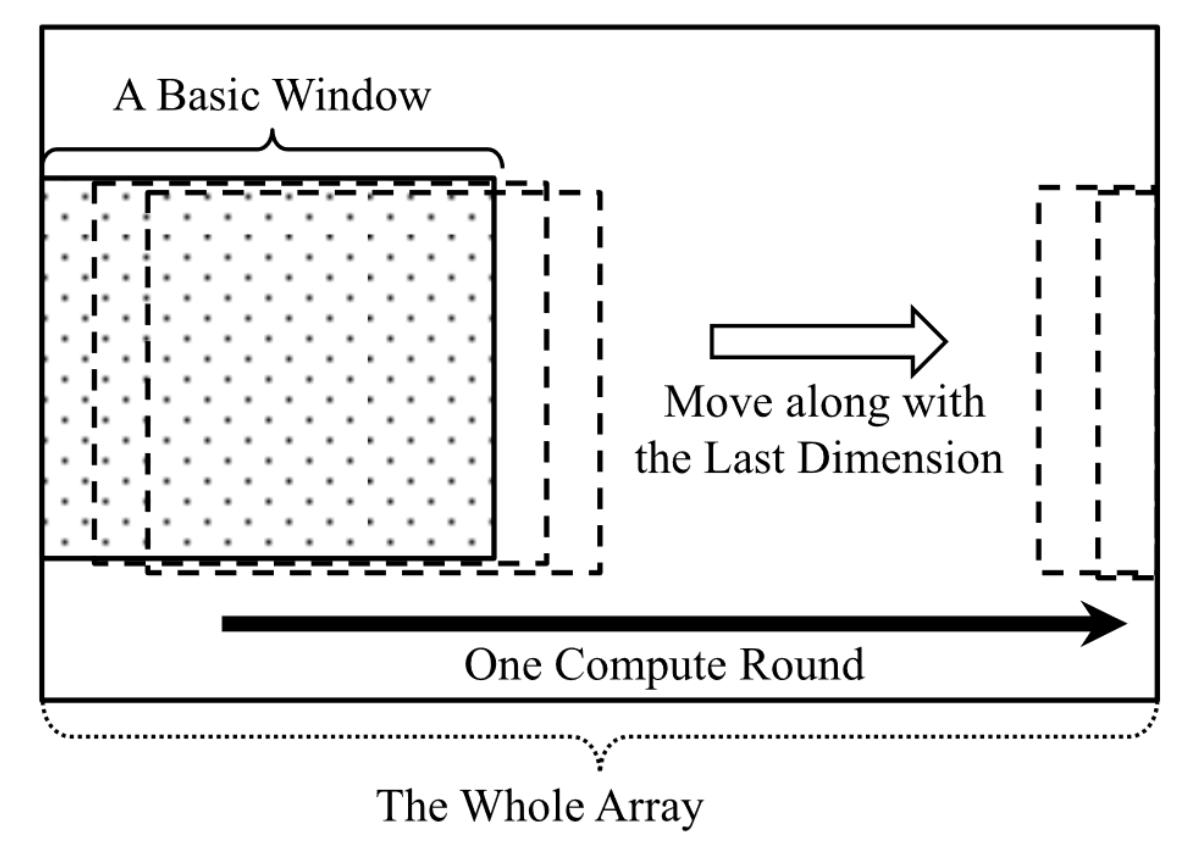
\includegraphics[width=0.6\textwidth]{windowAM.PNG}
\caption{Example of a sliding window \cite{windowAggr}. }
\label{windowAMwin}
\end{figure}

Sum and average operators are very similar as average uses sum and divides it by number of the elements. Because of this there will be only sum operator explained. This operator reuses SUM computed in previous windows by creating list structure (SUM-list) which contains sum values of every window unit. It generates basic window, computes its sum and initialize sum-list. Then it moves the window along with the last dimension with one step on one window unit, scans it and calculates the sum and updates the sum-list. Then it proceeds forward and continue to move the basic window down to obtain new ones. An example of creating and moving the SUM window can be seen in the pictures \ref{windowAM1} and \ref{windowAM2}.

\begin{figure}
\centering
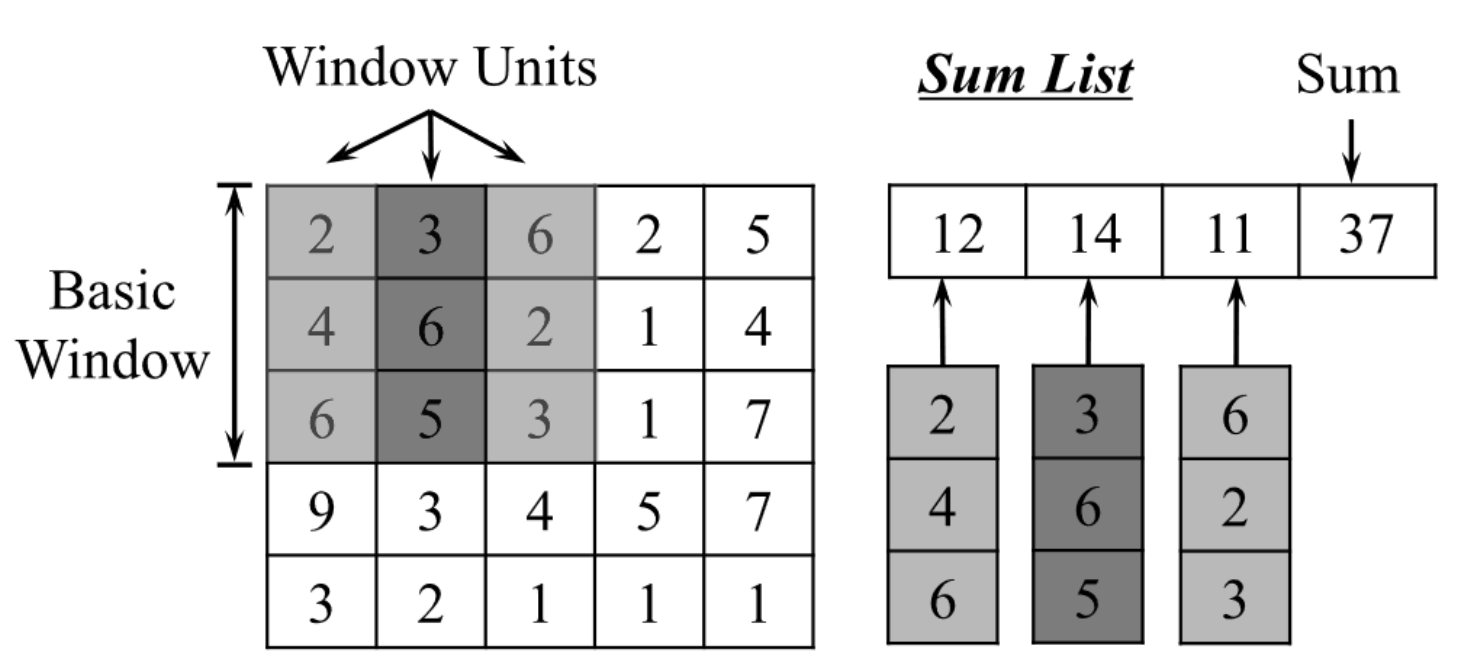
\includegraphics[width=0.7\textwidth]{windowAM_sum1.PNG}
\caption{Initialization of SUM window \cite{windowAggr}.}
\label{windowAM1}
\end{figure}

\begin{figure}
\centering
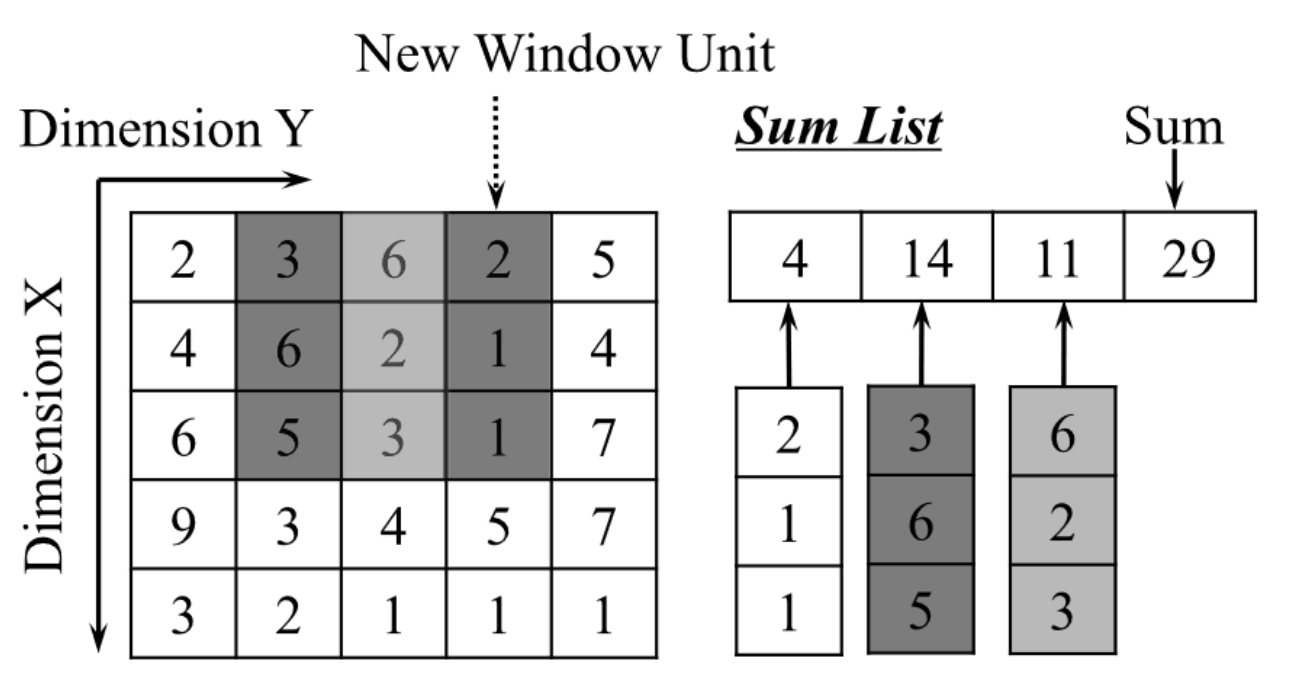
\includegraphics[width=0.63\textwidth]{windowAM_sum2.PNG}
\caption{Processing of a new unit and updating sum-list \cite{windowAggr}.}
\label{windowAM2}
\end{figure}

Min and max operators are handled by creating a heap data structure. The operator will generate basic window and scan window units in it and compute MIN/MAX for each one while inserting them into MIN/MAX heap. Then it moves the window along with the last dimension, obtains new window, calculates new MIN/MAX and insert it into MIN/MAX heap again. Finally it checks the heap root and removes it if its corresponding window unit is no longer present in the current window (this step is repeated until it corresponds). Proceed forward and calculate MIN of all windows derived while continuing to move the basic window down.

Percentile operator is a bit different from operators above. it is counted as $n=(P/100)*N+1/2$ and its structure is Self balancing binary search tree (SBST). Steps are: generate basic window, initialize SBST, insert all the values of the basic window into SBST, move the window forward along with the last dimension, insert new elements into SBST and delete old ones (i.e. ones not longer present in the current window). Then move forward and proceed to new basic window. \cite{windowAggr}


\section{Multidimensional Approximate Pattern Matching}
Solution of this problem can be used in the field of text searching, pattern recognition or computational biology.
First and easiest approach is to compute the Edit distance between the pattern and data but it can be used only when the problem consists of one dimension and it computes exact pattern match. Another solution (this time for approximate match) can be performed by dynamic programming which tries to find all segments whose edit distance to pattern is maximally k, where k is greater than zero and lesser then complete match. This solution can be improved by filters.

When the problem consists of two dimensions there can be uses a variety of methods. Subset of this solutions works only for string data and the main algorithms were developed by: Bird and Baker, Amir and Landau, Zhu and Takaoka, Karkkäinen and Ukkonen.

Scientists Krithivasan and Sitalakshmi developed The KS model which given two images of the same size, the edit distance is the sum of the edit distance of the corresponding row images. When used for approximate matching the sub-image of size $MxM$ is searched into a large image of size $NxN$, where they are using a generalization of the classical one-dimensional algorithm.

When fast searching under the KS model patterns and texts are rectangular. Special distance measure allows errors along rows but not along columns. Variations of this model are Exact Partitioning which is best for larger patterns, Superimposed Automata which is best for small patterns, Counting is best for small patterns and One error. There are two useful functions defined for this model. First of them is C(m,k,r) function which defines cost per text character to search r patterns of length m with k errors, and second is L(m,r) function that says the value for k/m where the one dimensional algorithm does not work anymore.

Another option to solve this problem is R model where each row is treated as a single string which is compared to other rows using one dimensional algorithm. Whole rows can be inserted and deleted. Modification of this model is RC model. If this algorithms encounter more than two dimensional problem it can be functional only if it has two hypercubes to compare which are reasonably close in size.

%\subsection{Approximate array pattern matching}
%This is a special case on the field of searching problems where user defines template pattern, similarity measure and an error bound. The algorithm then tries to find a set of locations where the distance in the array is closer to the patter then the given error. However these algorithm have problems such as complexity or processing of big data.

\subsection{Multidimensional Searching Algorithms}
To search across multiple dimension there are various algorithms to use, four of them are mentioned here. First of them is Exact Multidimensional Pattern Matching which divides the space along one dimension to obtain patterns of one dimension less. Then it searches all sub-patterns in each of the dimensional subtexts.
Second one is Fast filter for multidimensional approximate searching. This algorithm splits pattern across every dimension and then it searches sub-patterns the same way as exact solution, but all solutions found are checked by using the dynamic programming. Third is A stricter filter which says that whenever a piece appears the neighborhood can be checked. Its phase of finding possible solution positions is the same as in the previous algorithm but before checking the neighborhood with the use of dynamic programming the phase known as \textit{preverification} happens, in this phase all pieces of the pattern are checked one by one to see if they match where they should and only when finding sufficient number of pieces (i.e. size of the pattern minus errors that can happen along every dimension) that fit exactly then dynamic check can happen. Last algorithm presented is focused on adapting the filter to simpler distances. \cite{mdApproxPM}

These algorithms were not implemented by anyone yet, but I will provide detailed description of my solutions in section Implementation.

\section{Machine Learning Based Methods}
Main use of Machine Learning methods is in situations when in need of data analysis because people can often make mistakes, which make it difficult to find certain solutions.
These methods can be successfully applied in these situations and improve both the system efficiency and machine design. 

By working with the same set of features (here attributes) these algorithms can be even used when trying discover new data dependencies, classes and patterns. \cite{mlbm}
\subsection{KNN}
KNN or k Nearest Neighbors algorithm is very simple method of classifying items based on their distance to the pattern. The main goal of this procedure is to find \textit{k} nearest neighbors to the wanted item and classify it by the major class of its neighbors. This method is widely used since the 1970 and its one of the first and effective methods used for data mining.

First KNN algorithm was based on the Euclidean distance between the items, but it is possible to use other similarity measures (i.e they must meet the 4 basic criteria). Among the most widely used metrics belong: Euclidean distance, Kullback-Leibler distance, chess distance, Manhattan distance and Minkowski distance.

This approach is also known as similarity search, proximity search or close item search. Alternative way is introduced in \textit{R}-near neighbor search which is using a fixed radius. This algorithm tries to find all items that are within the distance \textit{R}. \cite{hashing}

One of the usable methods for solving this problem is using the Locality Sensitive Hashing.

\subsection{Kernel based methods}
Most of the machine learning based algorithms was developed for the usage in linear spaces while real word data often require nonlinear methods for dependency detection. By using kernel methods the dimensionality of the space can be reduced to a dot product. In this case the product acts as a similarity function between the pairs of data. The existence of a product like this enables these methods to act without computing the coordinates of the data but only computing the similarity between all of their pairs. Another advantage is that it is usually cheap to compute.

Among the algorithms using this method belong Support Vector Machines, Principal Component Analysis, Ridge regression, Linear Adaptive Filters and others. All linear models can be changed into non-linear by using kernel functions instead of its predictors. \cite{kernel} \cite{machineLearning}


\section{Adaptive Mesh Refinement}
AMR is a function with input parameters of Interval of values, spatial selection and its output is a set of cells with its values. To be returned by the function the cell must satisfy three conditions which are:
\begin{itemize}
\item cell must be uncovered
\item cell belongs to the spatial selection
\item value of the cell belongs in the Interval of values
\end{itemize}
AMR structure is contains of levels and refinement ratio. \cite{AMRindexing} First (coarsest) level is a box (defined by lower and upper corner). Every level can be decomposed into a disjoint union of boxes. A cell contains a pair of information and that is level it belongs to and its position by coordinates. By uncovered it is meant that the cell lies in the last (the least coarse) level. Spatial selection needs to be interpreted within the coordinate system of the first level and a cell in the spatial selection if its coordinates belongs inside the first level selection. Interval of values is simply the interval of values that the elements inside AMR structure can have. Values returned by function are in the pair with structure <cell, value>.

Construction of AMR Index tree consists of two phases where in the first one the object is split into boxes which create first level and then in the potential valuable boxes creates another level by splitting the box into smaller ones and so on, if the splitting is needed. In the second phase it creates a tree for every box which is covered by another (smaller) boxes.
%1. faze:
%rozdeli objekt na boxy, ktere tvori pocatecni vrsrtvu a pak v kazde dalsi vrtstve rozdeli nektere boxy na mensi, pokud je v danem boxu dalsi deleni treba. 
%2. faze:
%Vytvori strom  pro kazdy box, ktery je covered dalsimi (mensimi) boxy

The query process itself then first of all filters boxes that do not belong in the spatial selection, then filters boxes which values are outside of desired interval of values and finally it filters covered boxes as in the result it is required to have only uncovered boxes that belong to the most refined level.

\begin{figure}
\centering
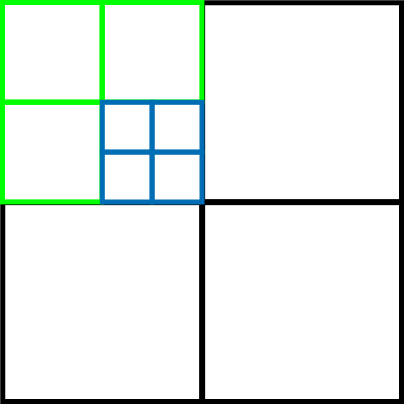
\includegraphics[scale=0.5]{amr_obr.png}
\caption{Example of AMR decomposition, different levels are represented by different colors}
\end{figure}

\section{Medial Axis Transformation}
Before defining Medial Axis Transformation (MAT) there is first needed to explain what a \textit{disk} is.
Disk is some specified shape or neighborhood of some specific point and it also has a radii, it belongs in the object and can not reach out of the object bounds. Object can then be defined as the union of the maximal disks it contains.

Medial axis transform of S consists of the centers of these disks together with their radii. The distance of a point x in S from S is then the length of the shortest path from x to the complement S. MAT can also be defined as the set of all points in S which do not belong to the minimal path of any other point, together with their distances. This can be imagined like constitution of a skeleton.

Each object is then defined by the triple $(c, d_c, w_c)$ where $c$ is the cell, $s_c$ is the largest square in which it is contained with width $w_c$. Set of these triples is called MAT of object S. This is very compact method for simple shapes.

In the field of digital pictures disks are approximated by squares and their orientation depend on the definition of grid distance, which also defines the type of the skeleton.

\begin{figure}
\centering
\begin{subfigure}{.5\textwidth}
 \centering
 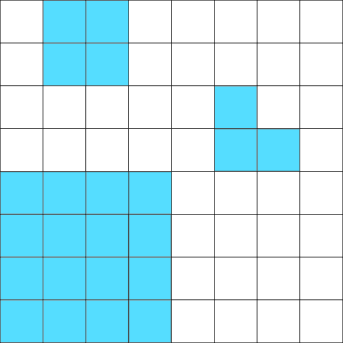
\includegraphics[width=.5\linewidth]{MAT_todo.png}
  \caption{Objects and cells that MAT algorithm will be performed at}
  \label{fig:sub1}
\end{subfigure}%
\begin{subfigure}{.5\textwidth}
 \centering
 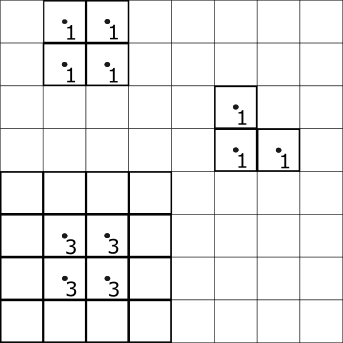
\includegraphics[width=.5\linewidth]{MAT_done.png}
 \caption{MAT for the collection of objects and cells, maximal block is anchored at the unit-size element at its center}
\end{subfigure}
\end{figure}

Base types of distances that can be used are:
\begin{itemize}
\item Chess-board distance - disks are upright squares
\item city block distance - disks are approximation of diagonal squares
\item Euclidean distance - disks are discs, also more appropriate in continuous space
\item Absolute value distance - disks are diamonds
\end{itemize}

When using irregular grid it can decompose the space using hyperplanes resulting in collection of blocks. By this there can be recreated irregular block sized grid, where no recursion is involved and block decomposition is handled by explicit representation. These blocks are not congruent (this will add access structure containing linear scales which indicates position of partitioning hyperplane).

Representation of block decomposition can be done by using different types of quadtree or octree. Most commonly used decompositions are:
\begin{itemize}
\item Multicoloured quadtree - can contain more than two colours and also more block labels
\item Binary quadtree - for black and white values only
\item Block specified by a pair of coordinates - specified by upper left corner coordinate and size of the side
\item Morton block - encoded by localization code (variant of Morton number), which is power of two and Morton ordering is NW, NE, SW, SE
\item Scan of resulting representation from extreme right end to first zero valued bit
\item Sorting the values in increasing order - Efficient pixel interleaving compression technique (EPICT)
\end{itemize}
\begin{figure}
\centering
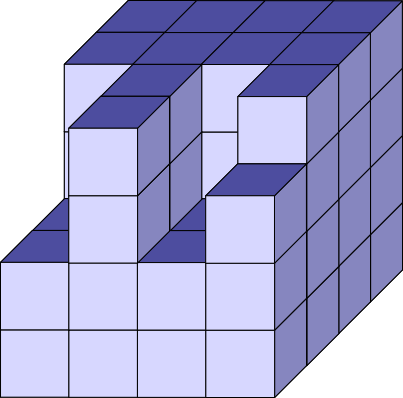
\includegraphics[scale=0.5]{mat3d_todo.png}
\caption{Object that block decomposition will be used on}
\end{figure}
\begin{figure}
\centering
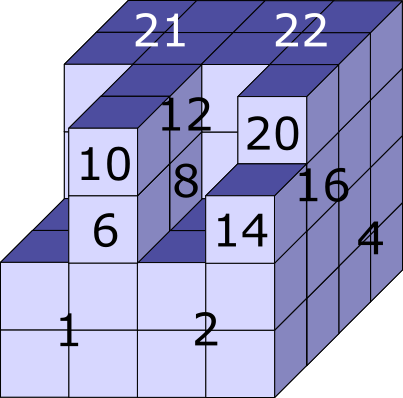
\includegraphics[scale=0.5]{mat3d_todo_numbered.png}
\caption{Region octree block decomposition of the picture above}
\end{figure}
\begin{figure}
\centering
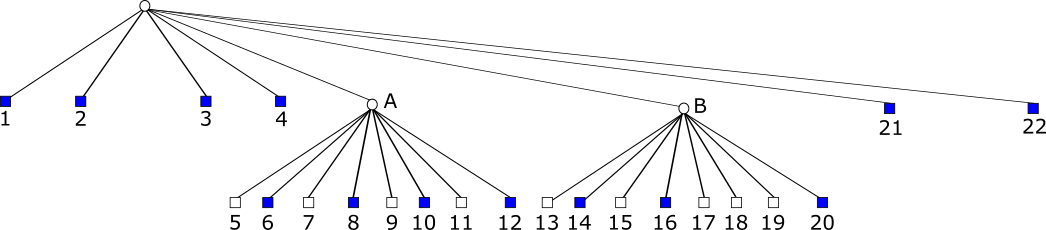
\includegraphics[width=\textwidth]{mat3d_strom.png}
\caption{Octree block decomposition of the picture in Figure 1}
\end{figure}

Typical usage for this algorithm is at nearest neighbor finding query.
In this task the goal is to locate neighbor of the element, which can be done by following ancestor links until finding nearest common ancestor and then descending to the leaf.
For this task there can be used the Spaghettis algorithm \cite{spaghettis} which has only one parameter and it is the number of pivots used. As because the parameter it is clear that the algorithm is pivot based, mapping metric space to k-dimensional vector space. Its competitive algorithm is AESA (Approximating Eliminating Search Algorithm). The distance function of this algorithm has metric properties. Similarity queries solved can be divided into two categories and these are range queries (retrieve all elements which are within distance r to q) and nearest neighbor queries (retrieve the closest elements to q in U). The algorithm steps are: For each pivot calculate and save the distances to each database element. Sort each array saving the permutation with respect to the preceding array (from array to array only the successful traversals are followed). Given k intervals, define k sets (k is number of pivots). Obtain the index intervals corresponding to each set and follow each point through the pointers to find out if it falls inside all the index intervals. If a point falls inside all the index intervals it is in the intersection.

There is also a modification for nearest neighbor queries by selecting unchecked point do range query and if it returns more than one element repeat with lower range else stop. In this case random selection is not totally ineffective.
\subsection{Types of MAT}
There is range of types of MAT algorithm, varying from different measures to data organization.
\subsubsection{SPAN}
The Spacial Piecewise Approximation by Neighborhoods is the generalized version of MAT algorithm trying to compute maximal homogeneous disks. It is the same for pictures with two values (white/black) as there it is looking for constant values. But it is expensive to compute.
\subsubsection{GrayMat}
This algorithm uses Gray-weighted distance. To use it effectively there is a need to segment the picture into two classes. First class is marked as 0 (e.g. background of the picture without objects) and second class is labeled as non 0 (e.g. objects in the picture, not the background).
\subsubsection{GradMat}
In this approach there can be computed a specific score for each point P of a picture based on the gradient magnitudes at all pairs of points that have P as their midpoint. These scores are high for points that lie midway between pairs of anti-parallel edges. They define a weighted "medial axis". 
Advantage of this algorithm lies in its sensitivity to noise and irregularities in region edges.
\subsubsection{MMMAT}
This variation of the MAT uses Min Max algorithm and is insensitive to noise. It is based on the fact that the MAT of a set S can be constructed by a process of iterative shrinking and re-expanding which corresponds with local MIN and MAX operations. When this construction is used it can be applied to gray-scale pictures. \cite{MMMAT}
\subsubsection{QMAT}
Mentioned method is appropriate for processing pictures containing only binary values. It can be imagined that this picture is like an array of $2^n x 2^n$ pixels, which id going to be repeatedly subdivided into quadrants until blocks which consist of a single value are obtained.
Quadtree skeleton then consists of the set of black blocks in the image satisfying three conditions and its radius. The conditions are:
\begin{itemize}
\item Whole image is spanned by the skeleton
\item Elements of skeleton are the blocks with the largest distance transform values
\item No block in the set of blocks but not in the tree requires more than one element of the tree for its subsumation.
\end{itemize}
Each created tree is unique and also has distance value stored in each black node (in white nodes there is no need to store it as there would be 0 value).

\begin{figure}
\centering
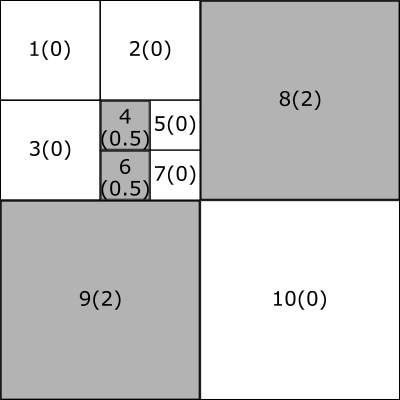
\includegraphics[scale=0.5]{qmat_picture.png}
\caption{Sample Image}
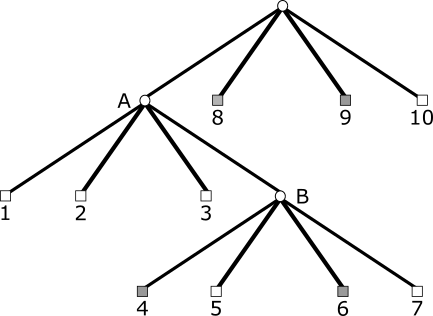
\includegraphics[scale=0.5]{quadtree.png}
\caption{Quadtree of the Sample Image}
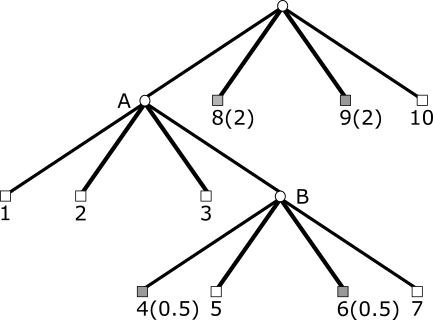
\includegraphics[scale=0.5]{QMATtree.png}
\caption{QMAT tree of the Sample Image}
\end{figure}

\section{Knuth--Morris--Pratt Algorithm}
This algorithm was first presented in 1977 by scientists Knuth, Morris and Pratt \cite{kmp}. In their work they describe new algorithm usable for a string searching. The main idea of it is to remember for each position of the pattern P the length of the longest suffix P which matches to the prefix of the P. unlike the naive algorithm that after every mismatch shifts only by one position, which causes some parts of the data to be read again, KMP notices that it is possible to 
move by more than one position, this information is gained when comparing previous characters. To be able to remember all the extra information the algorithm uses is stored in a pre-computed table.


\section{Similarity join}
This join can be used on array data model which means a model where multidimensional array is defined by a set of dimensions and a set of attributes. Each dimension is a finite totally ordered discrete set and all cells in a given array have the same type. It must allow chunking and have shared-nothing architecture. Array join is a join of dimensions and union of attributes. The goal of the similarity join is to find all the pairs of points such that the distance between them is smaller than some Epsilon.
When applied on arrays the result dimension is union of joined arrays dimensions, result cells are the ones satisfying the given condition ($k=j+l$ in the picture), this can handle arrays with various dimensionality. Most general algorithm used for this is nested loop join. \cite{simJoin}
\begin{figure}
\centering
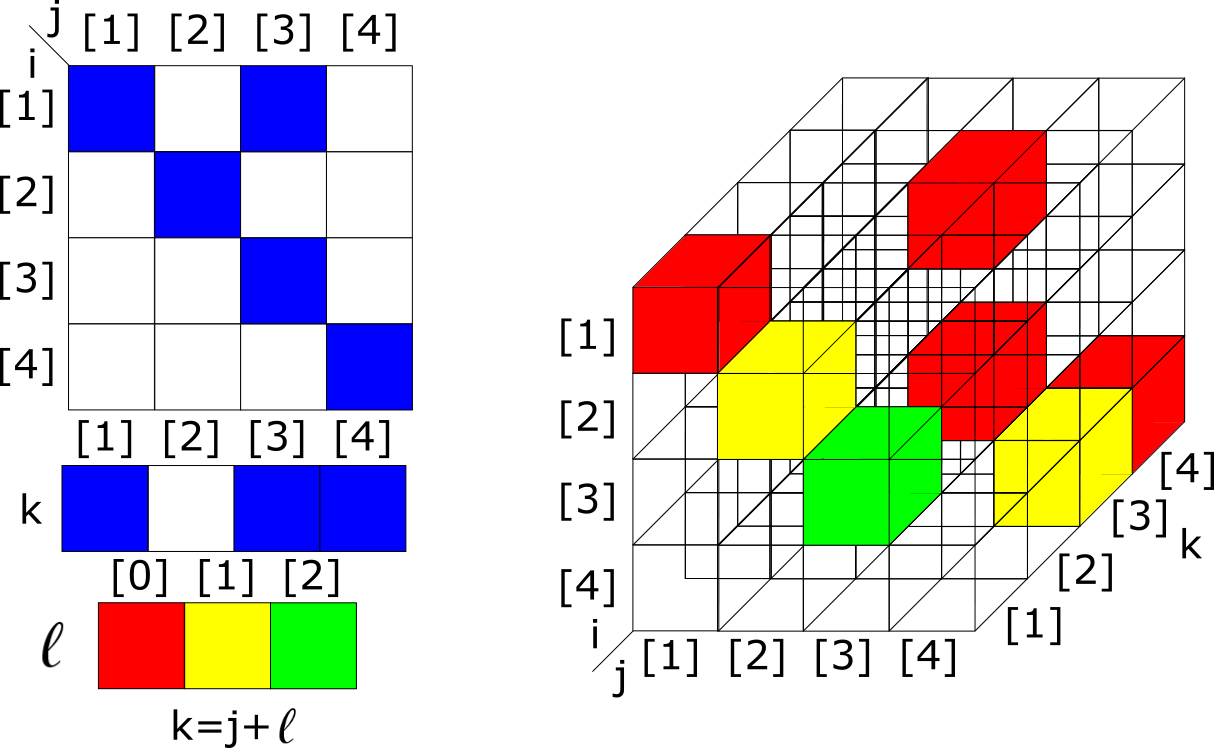
\includegraphics[scale=0.4]{simjoin.png}
\caption{Similarity join of 2 different arrays, first 2 dimensional, second 1 dimensional with condition array $\ell$. Result is in the 3 dimensional cube.}
\end{figure}

\section{Computing marginals using MapReduce}
As a marginal of a data cube it can be understood the aggregation of the data in all those tuples that have fixed values in a subset of the dimensions of the cube. Order of the marginal is the number of dimensions over which aggregation is happening. Mapping of reducers q and replication rate r is that no reducer associated with more than q inputs and for every output there is some reducer that is associated with all the inputs that output needs for its computation. Dimensions in this case have same number of different values.
Function C(n,m,k) defines minimum number of sets of size m out of n elements that every set of k out of the same n elements is contained in one of the sets of size m, and it is called the covering number.
Different sets of n,m,k are handled differently but when approached with unknown values it can be solved as: one group of handles contains dimensions to m-k+1 plus any k-1 dimensions from group 2, and others are formed recursively to cover the dimensions of group 2 and have none of the members of group 1.
This problem can be generalizes as a problem with weights of dimensions and dividing dimensions into several groups. \cite{marginals}

Example of computing marginal in three dimensional space (as seen in the pictures 10 and 11):\\
SELECT SUM(V) \\
FROM DataCube \\
WHERE D1 = x, D2 = y, D3 = z;\\
\begin{figure}
\centering
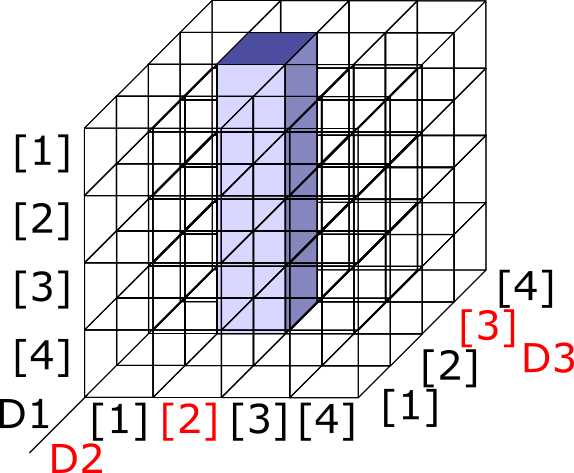
\includegraphics[scale=0.5]{marg1d.png}
\caption{Example of DataCube and selecting dimensions where y=2 and z=3}
\end{figure}
\begin{figure}
\centering
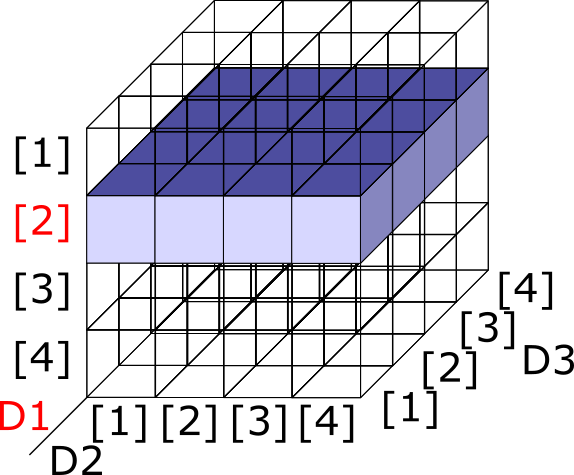
\includegraphics[scale=0.5]{marg2d.png}
\caption{Example of DataCube and selecting dimensions where x=2}
\end{figure}



\chapter{Implementation}
This chapter will discuss the implementation. It presents a variety of solutions ranging from brute force exact pattern matching, up to the more complex versions of approximate pattern matching.

Primary languages were C++ and Python. For compilation of *.cpp programs user needs at least compiler of version 2011 (flag \texttt{-std=c++11}). All python scripts were run using version 3.0. A \textit{numpy} library is also needed. A \textit{Makefile} was created in order to simplify the C++ compilation.

Libraries used in C++ were iostream, fstream, string, vector, math.h and chrono which are all included in the C++11 standard.

When running the created C++ executables it can be done by command:

$$./executable\_name\quad input\_data\quad input\_pattern.csv\quad errors$$  

where input data have to be chunked and name of the meta file is expected, input pattern is a standard csv file with the specified dimensions and attributes, errors is a parameter used only in executables of approximate searches and defines maximum number of errors allowed for the result to still be valid.

\section{Output Format}
After successfully running the executables in the terminal window the program will write in the standard output stream. First it will write Finding, meaning that the part of the program that searches for solutions started and all initial settings and reads are done. When finished with find phase program will output the time it took to find the results and after this it will write coordinates of the found solutions. They will be written in the form of list of all possible dimension coordinates where the desired pattern can be found while not violating the constraint about maximum number of errors.

Usual output would contain an array of found solutions, however as this work is concerned about the process of finding, the result serve mostly a confirmation role. If the algorithms were used in real system, it would be simple to modify the output to suit the system needs.

\section{Input Data}
A large part of the database search revolves around used data structures, so this section will focus the specifications of used formats and other properties.

\subsection{Format}
Data format (file extension) that can be successfully processed is of types CSV and BIN where CSV data must have a header in the format:
\begin{itemize}
\item 0:DIMX$_0$, 1:DIMX$_1$, ... , N:DIMX$_N$, ATTR1:TYPE, ATTR2:TYPE, ... , ATTRL:TYPE
\end{itemize}
In this format $(0, N)$ is an order of the dimension whilst $(X_0, X_1, ... , X_n)$ is a number of unique values that are in this dimension. $(ATTR1, ATTRL)$ specifies the name of the attribute and TYPE parameter contains the type of the values in the attribute, only one type per attribute is allowed. Currently the program is optimized for integer attributes, every other type would be processed as a string.

When the user needs binary data, Python script named: \textit{chunk.py} can be used to create chunked and binary data from the original CSV file. Usage of this program is specified in the next section called Chunking.

Following this specific header are usual CSV data. Be aware that the data can be sparse, which means there can be missing cells or attributes.

\subsection{Generating Data}
Data generating is taken care of by two Python scripts where both of them generate hyper-cubic data (this is a simplification for the analysis of the algorithms, although algorithms can be used for different lengths of dimensions and patterns). First of them named \textit{generate.py} and can be used with the command:

$$ python\quad generate.py\quad dimensions\quad length\quad attributes\quad value\quad out$$

Where dimensions is a number specifying how many dimensions should be generated, length is a size of one dimension, attributes specifies a number of attributes there will be whilst value notes maximum value allowed in the attribute. Parameter out means the name of output file to which the data should be generated. This script will generate data where no cell is missing or NULL value.
When in need of sparse data, second script named \textit{generate\_Gauss.py} can generate them with the help of multidimensional Gaussian functions. Command to run this script is: 

$$python\quad generate\_Gauss.py\quad dim\quad length\quad density\quad results\quad pSize\quad pFile\quad output$$ 

Where dim and length have the same meaning as in the script above, density says the ration between generated and empty cells (value from interval <0,1> is expected), results means how many results should be generated in comparison to the size of data, value from interval <0,1> is expected as it is approximate chance for the pattern to be generated. Parameters pSize and pFile specify the size of the pattern in one dimension and the input file with the generated pattern (CSV file is expected). Output parameter means the name of a newly created file with generated data.

The actual generating is based on three Gaussian distributions with the centers set in three different positions:
\begin{itemize}
\item All coordinates at the third of the current dimension size
\item Coordinate in first dimension at the third of first dimension size and rest coordinates at half of the current dimension size
\item First coordinate at position of two-thirds of the first dimension size, all other coordinates at position of five-sixths of current dimension size
\end{itemize}

\subsection{Filtering}
Python script \textit{filterPattern.py} is ideal for creating patterns at specific positions of the data. When in need of a particular pattern that needs to be at the exact position in the data this program can be run using the following command in terminal:

$$python\quad filterPattern.py\quad input\quad DIMS\quad LENGTHS\quad ATTR\quad output$$

Meaning of the parameters are: input specifies the input file (expected CSV) from which the pattern should be generated, DIMS is a list of all dimensions that need to be included in the pattern where the value (0, length of the dimension) on each positions signifies start position of the pattern in every of the included dimensions. Parameter LENGTHS specifies another list, with the same length as the previous one, where each number (0, x) means the length of the pattern in this dimension from its start position, $x$ is smaller than the length of an associated dimension minus start position in the same dimension. Next there is parameter ATTR where value $0$ or $1$ is expected, this number says if the attributes should be kept or not ($0$ for NO, $1$ for YES). Lastly there is the \textit{output} parameter where a suffix is expected, this string will be added at the end of the original file name...

\subsection{Chunking}
All tested data are represented in binary format and chunked into files which represent a set number of cells based on the dimension sizes. Chunks are created by using the attached Python script \textit{chunk.py}. This script can be run by using the command:

$$python\quad chunk.py\quad input$$

where parameter input specifies input file that should be chunked. When successfully finished the script will create certain number of binary files based on the length and number of dimensions and also number of attributes.
Attribute values are added into the relevant file, which is determined by the dimension values. Created files have their names same as the input file with the dimension numbers added to signify which data are stored in them.

As was already specified SciDB has its own binary format and the chunking uses exactly the same format. This means there is always one special file with meta information about the chunked binary files. In meta file there can be found header of the original data as this file is not binary encoded. There is also a mask file that specifies if a cell is in the data or not by using one bit per each cell (0 means the cell is not in the data and vice versa). Other files created by the script \textit{chunk.py} are binary files that contain a sequence of cell values. For the sake of testing attributes were only of integer type, but implementation can also work with string values. All of the integer values were smaller than $2^{16}$ so they would fit into 2 bytes.

\section{Exact pattern matching}
Every other algorithm is a type of pattern matching. This section will present implemented exact solutions. Exact pattern match means there are no errors and the pattern is present in the data without changes. Two solutions were implemented as reference solutions. First of them is solution using naive brute force algorithm. Second is algorithm by Navarro which skips first dimensions and thus have smaller both patterns and data to compare.

\subsection{Brute Force}
As the name suggests this algorithm goes through every position in data and starts to compare the pattern from the ``top-left'' corner until it encounters error. This solution is very simple, on the other hand there is obviously no possibility not to find every position of the pattern.

Just to clarify things, the algorithm iterates over every dimensions and in it over every values, thus the returned positions are sorted.

\subsection{Baeza-Yates and Navarro modification}
This algorithm was proposed by Baeza-Yates and Navarro \cite{mdApproxPM}. Its process is similar to the brute force algorithm, however one dimension which is present in both the pattern and the data is selected. While iterating through this dimension instead of taking steps of length 1, steps of length $m$ are taken.

Not to miss any possible solution, every ``row'' of pattern is compared with the given part of the data. This process is better illustrated in the figure \ref{fig_skipDim}.

\begin{figure}
\centering
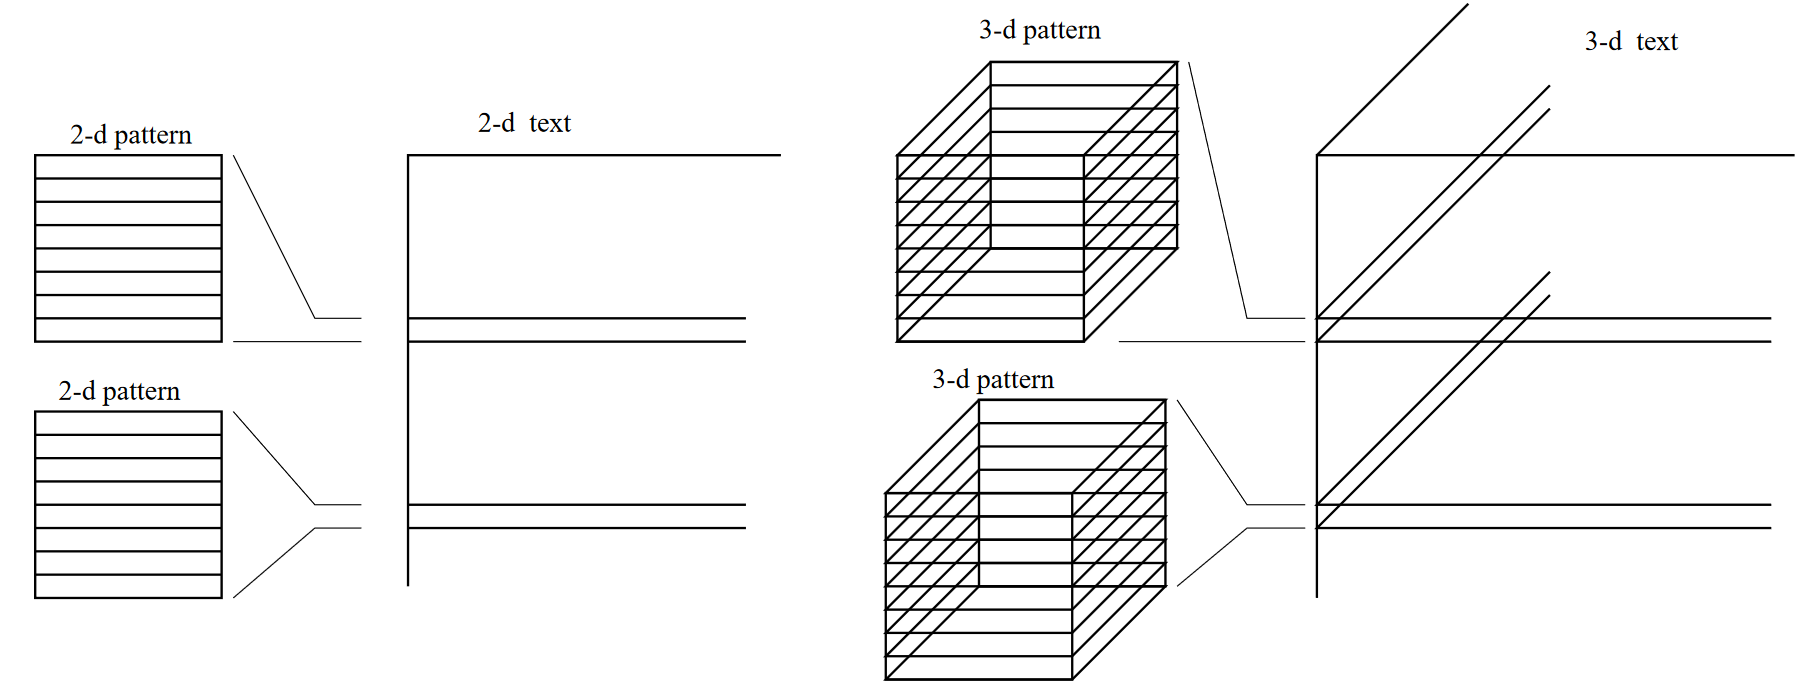
\includegraphics[width=\textwidth]{skipDim}
\caption{Skip dim}
\label{fig_skipDim}
\end{figure}

Considering that both pattern and data have all dimensions with the same sizes and the selected dimension is arbitrary, the first one is always used for easier implementation. This modification reuses parts of data instead of using every single cell.

\section{Approximate pattern matching}
Previous two solutions could us a simple identity function to recognize, whether the solution is valid or not. If an approximation is taken into account, the algorithm has to measure the difference between the pattern and the currently tested position. There exist several options to do that. In the next section all implemented variants are presented.

In every solution an input value $k$ is added, which represents the maximal tolerated error.

\subsection{Brute Force}
First and again the simplest solutions to iterate over every part of the data and compare one coordination of the pattern of another until either whole pattern is checked or the $k$ number of errors are found.

This method obviously always finds every valid solution so the False Negatives are 0. However it is linearly dependent on the selected error, so it is not suitable for large patterns with higher error range. On the other hand, the implementation is very simple again and it serves as a solid confirmation of the correctness of other solutions.

\subsection{Fast Filter Searching}
A less demanding solution was proposed again by Baeza-Yates and Navarro \cite{mdApproxPM}. Its idea is similar to the modification made in the exact algorithm, however in this case an iteration in all dimensions present in the pattern are influenced.

The data are virtually divided into sections, which are the same size as the pattern. The iteration through positions in dimensions not present in pattern is the same as in brute force algorithm. However in the other dimensions, both the section of data and the pattern is divided into the same number of parts and the comparison is made only between the ``bottom-right'' corner of data section and all pattern parts. Not to miss any possible positions, the compared part of the data has to be moved always by one cell part size - 1 times. Again, for better illustration a figure \ref{fig_slide} is provided. In the picture each part of the pattern is compared with every blue part of the data.

\begin{figure}
\centering
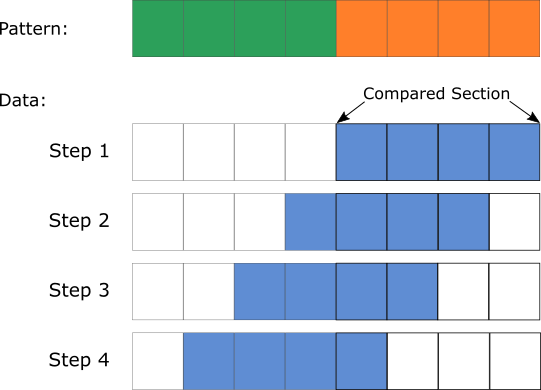
\includegraphics[width=\textwidth]{slide}
\caption{Example of sliding window.}
\label{fig_slide}
\end{figure}

In current implementation all dimensions are split into $m$ parts, except the last, which is split into $j$ parts, where:

$$j = \lfloor k^{\frac{1}{d-1}} \rfloor + 1$$

this value is recommended, so it was not tampered with. This relatively small parts are compared by basic identity function and the positive results are remembered. The whole process usually returns more results than it should, because only a small parts of the pattern are matched. So further verification is needed.

In this case a dynamic programming method is utilized. To perform the dynamic programming check, multiple approaches are available. Completely implemented and tested was only Edit distance, with framework prepared in code for R, C and RC measures. Following methods also use this step, so the dynamic programming was reused.

Usually the dynamic programming confirmation would be made right after finding each position. However considering that all implemented algorithm use chunked data and thus not every section of the pattern is necessarily in the memory, these stages are split and the whole data are searched through for the partial matches and after that the dynamic programming check is performed on all found positions.

\subsection{Stricter Filter}
A slightly modified version of previous method is called Stricter filter and was proposed in the same paper. The disadvantage of previous solution is, that if the first partial matching finds a large number of False Positives, the dynamic programming is then a bottleneck, because it is computationally expensive to perform.

Therefore, before the last stage a preverification step is added. It has the same goal as the dynamic programming, however is much simpler and thus much faster. It should filter a large portion of results, which will not be necessary to go through by the dynamic programming.

The idea is to check the found area cell by cell and remove it from solutions if more than $k$ are found. The preverification can end before iterating through all cell if:

\begin{enumerate}
\item $k+1$ errors are found, i.e. the position is not a solution.
\item Less than $k - q$ cells remain to compare, where $q$ is the number of already found errors.
\end{enumerate}

\subsection{Hashed Stricter Filter }
All of the previous approaches were either the simple obvious solutions or previously proposed by Baeza-Yates and Navarro. The last solution is built upon the Stricter Filter and modifies one significant feature. The problem with Stricter Filter solution is, that there has to be the partial identity for arbitrary error value.

So instead of using the comparison of the actual sections of pattern with the data a hash function is implemented. Firstly, all parts of the pattern are hashed, so it is done only once. The same cannot be done with the whole data as only some parts should be hashed and the data are not loaded at the start as they are chunked in smaller files.

Three similar solutions are presented:

\begin{itemize}
\item sim hash %TODO
\item sim hash once %TODO
\item rolling hash %TODO 
\end{itemize}

The rest of the process stays the same as in the Stricter Filter, so preverification and dynamic programming check is performed.

The assumption is, that the added hashing may increase the computation speed, because a lot shorter values are compared instead of whole sections. However the part size will have high impact on the improvement, because the higher the ratio between part size and hash size the bigger the improvement. Another possible outcome is to find even more partial results for preverification, because the the hash function will probably make some collisions.

The best case scenario thought is that the collisions will be for similar sections and thus possibly valid positions, which were disregarded by the Stricter Filter method. This is the reason for usage of Sim-Hash %TODO

\section{Possible modifications}
Some other modifications were considered and two of them were analysed, whether it could have a positive impact on already implemented solutions. First modification consist of changing the comparison between the section from the naive algorithm to KMP as the sliding part of the data may be considered as a longer array and the comparison could return only a position in the slide. However considering that the compared sizes are part size and 2 * part size - 1 long, and the non-repetitive type of data, the creation of the table T used in algorithm would add another space requirement and the speed increase would probably not occur, because mostly, the check ends after single value comparison. If these methods were used data, where a repetition of subsequences was expected and the part size was set to sufficient value, it may prove to be faster.

Second modification was to use hashing even for preverification stage. As the pattern was already hashed it seemed as a viable option. However the data were not hashed, at least not all parts of them, and the hashing would take similar time as the actual preverification, so it was not used. If the data were for some reason hashed before, the idea could prove more plausible.


\chapter{Results}
This chapter will focus on presenting and discussing the results of selected implementations. First part will discuss measured times and its dependency on size and density of the file, number of dimensions and number of pattern matches. For this task, 8 testing files were generated using the Gaussian generating script. Second part will focus on explaining memory usage and also demonstrates the quality of chunking algorithm.

\section{Time complexity}
Time measuring was done with the help of boost library, which belongs in the C++ standard since 2011. In the first graph \ref{fig_compT} there can be seen times of all implemented algorithms achieved for the input file with standard parameters and standard pattern of size $16\times16\times16$. This standard file was compared with all other files and its parameters were:
\begin{itemize}
\item size -- 256 MB
\item density -- 50 \%
\item number of dimensions -- 3
\item presence of pattern -- 0.1 \%
\end{itemize}

Abbreviations on the x axis correspond with these algorithms:
\begin{itemize}
\item BE -- Brute Force for exact pattern matching (EPM)
\item SE -- Baeza-Yates and Navarro algorithm (EPM)
\item BA -- Brute Force for approximate pattern matching (APM)
\item FFS -- Fast Filter Searching (APM)
\item SF -- Stricter Filter (APM)
\item HS -- Hashed Stricter Filter (APM)
\item HS1 -- Hashed Stricter Filter second implementation (APM)
\item HR -- Hashed Stricter Filter third implementation (APM)
\end{itemize}

Yellow color symbolizes the time needed for finishing of preverification and red color means the time of dynamic check.

\begin{figure}
\centering
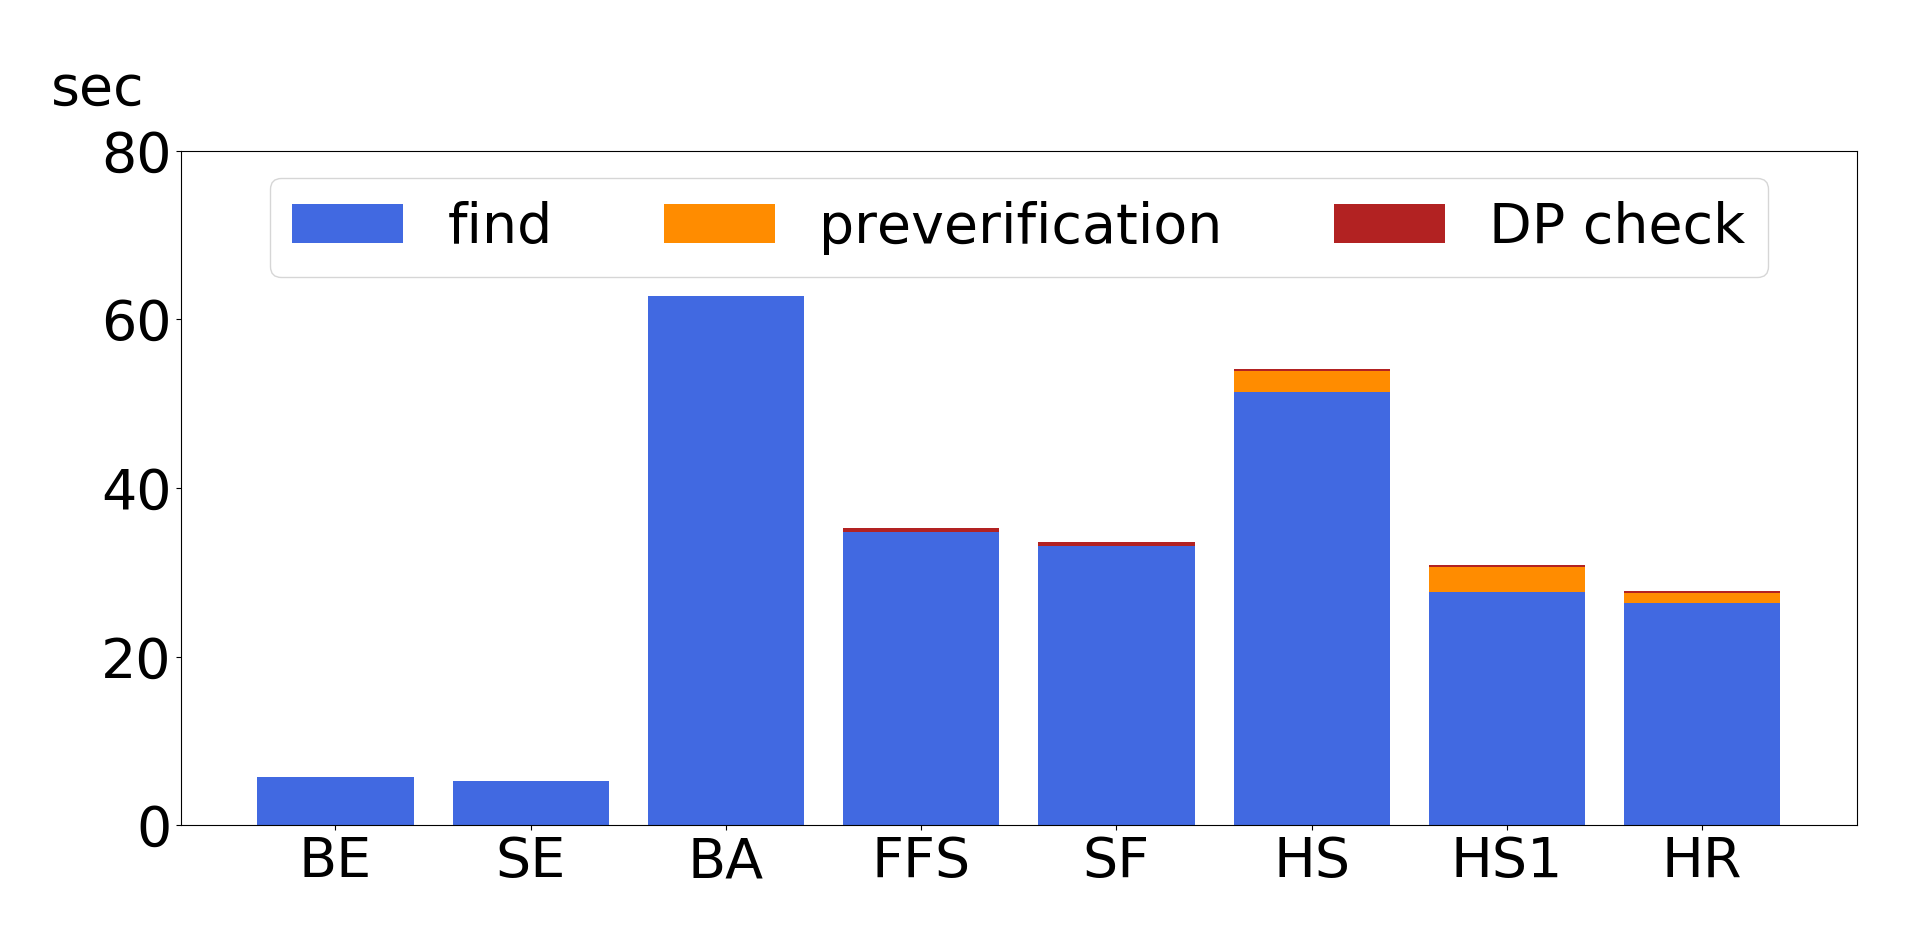
\includegraphics[width=0.8\textwidth]{img/baseAll}
\caption{Computation time for all implemented algorithms.}
\label{fig_compT}
\end{figure}

As can be seen in the graph, solutions of EPM achieve higher performance than APM solutions. This is because whenever exact algorithms encounter a mistake they can dismiss this possible solution while approximate approach has to control until $k$ mistakes are found. Because of this distinct difference exact algorithms are not considered in another graphs.

Another important thing to notice in the graph is that using the preverification before dynamic check visibly speeds up the whole control process, which is a difference between FFS and SF algorithms. 
%to je teda pekna blbost, protoze tam neni zadna preverifikace...zluta je preverifikace..melo by to byt stejny, asi jen chyba mereni

\subsection{Dependency on data density}
Measuring in this section was done using 3 different files. One of them is the standard file specified in the first section, other 2 files were different only in the density of generated data and its values were $100 \%$ and $2 \%$.

In the graph \ref{fig_densRes}, green color represents dense data, orange $50 \%$ density and blue $2 \%$ density. It is clearly visible that lesser the maximum error allowed the higher the dependency on the data density. Times achieved when allowing up to 4 errors is multiple times worse for the least dense data. This happens because when the density is low there is a lot of positions to check even when there are no data in them. 

However there can be seen that solutions using hashes can reach better times than other algorithms especially in the data with low density. Reason for this is that non-hash algorithms can take a while to reach a position with no data, but when using second and third implementation the overall comparison is quicker because the value of the hash is NULL if some of its value is not in the data. Which means that a lot more positions can be skipped directly.

Solution using variant of LSB hash can be very successful for low errors allowed but rapidly worsens with growing error rate. This is why there is such a peak for error 16 and also its time is not used in the last graph for better scaling. In the last graph the brute solution is also omitted.

\begin{figure}
\begin{minipage}{.5\linewidth}
\centering
\subfloat{\label{dens:a}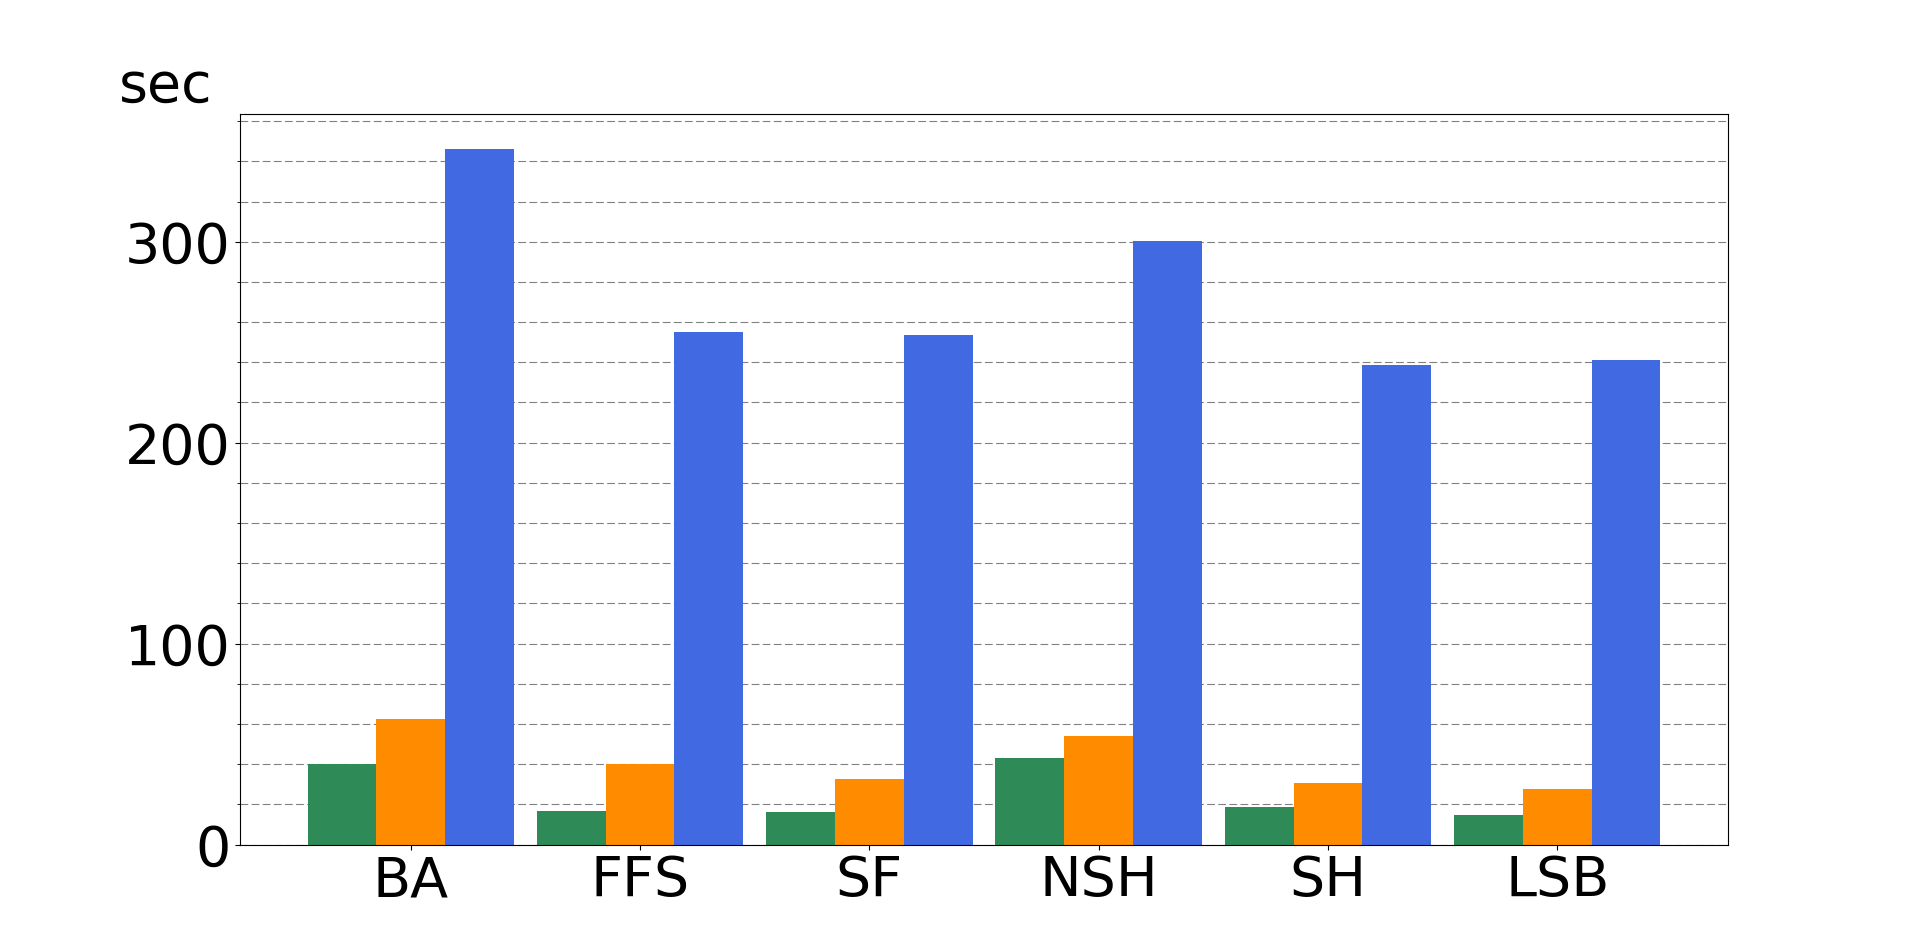
\includegraphics[width=\textwidth]{img/dens0}\caption*{Error = 0}}
\end{minipage}%
\begin{minipage}{.5\linewidth}
\centering
\subfloat{\label{dens:b}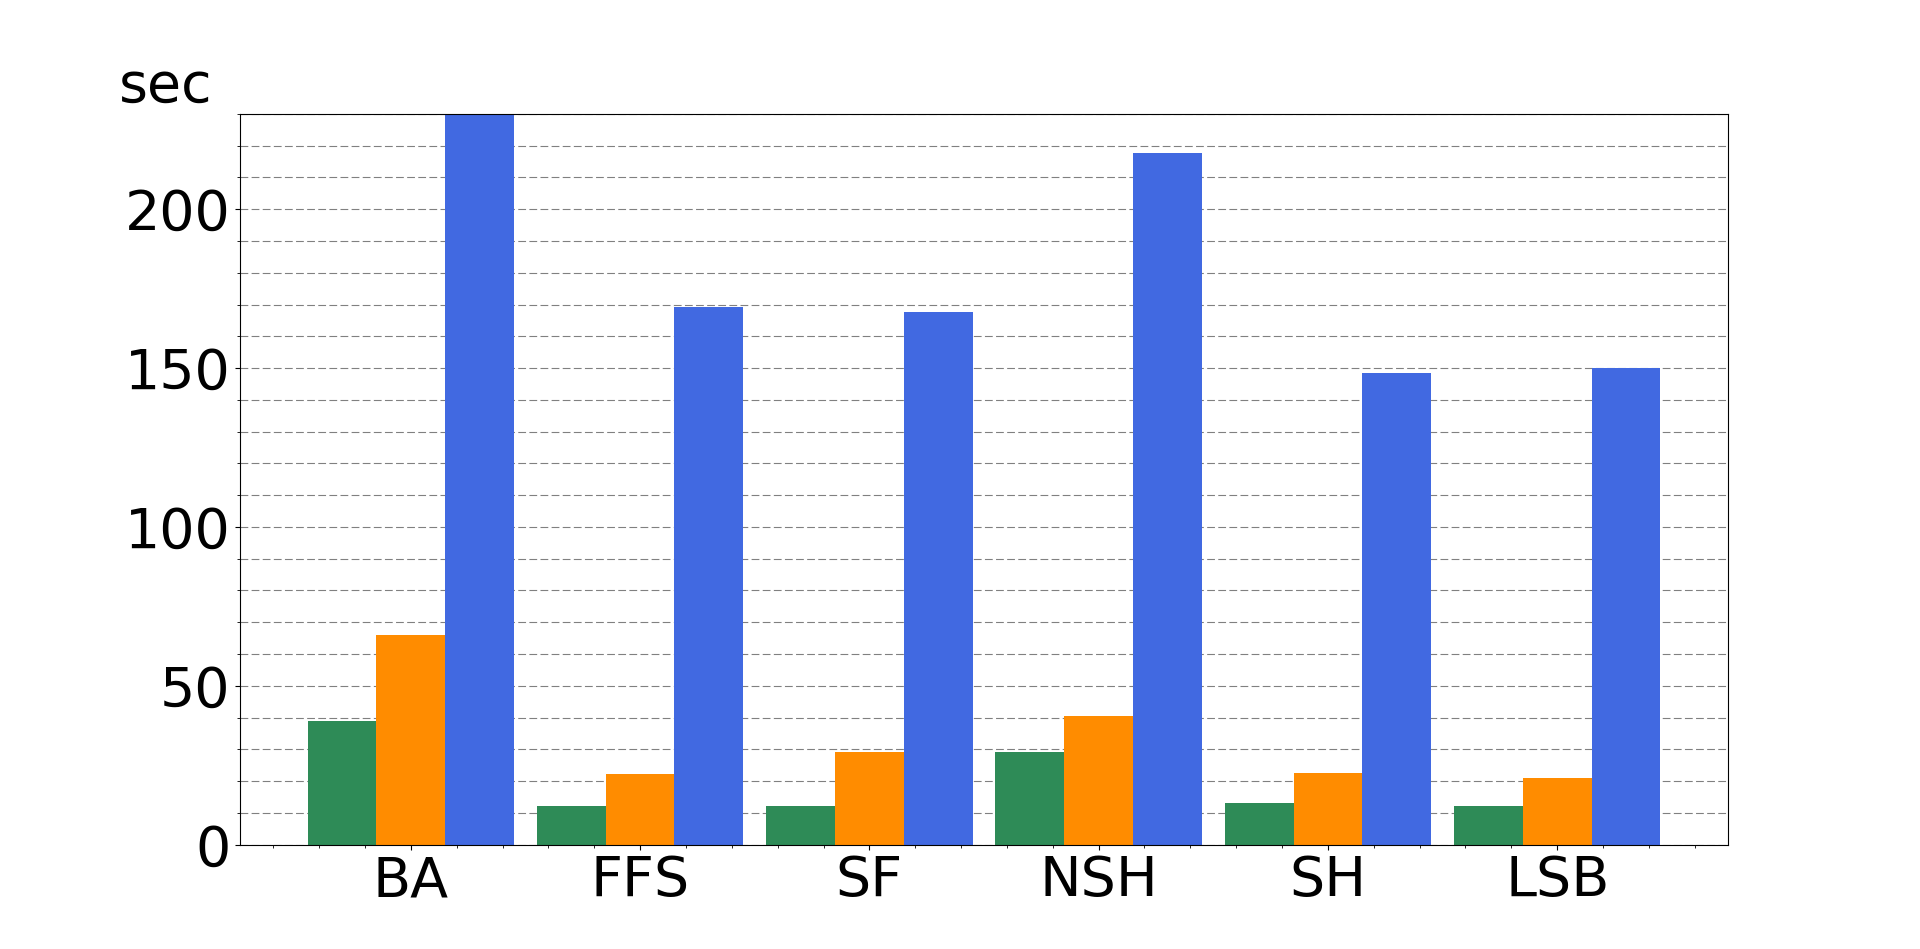
\includegraphics[width=\textwidth]{img/dens4}\caption*{Error = 4}}
\end{minipage}\par\medskip

\begin{minipage}{.5\linewidth}
\centering
\subfloat{\label{dens:c}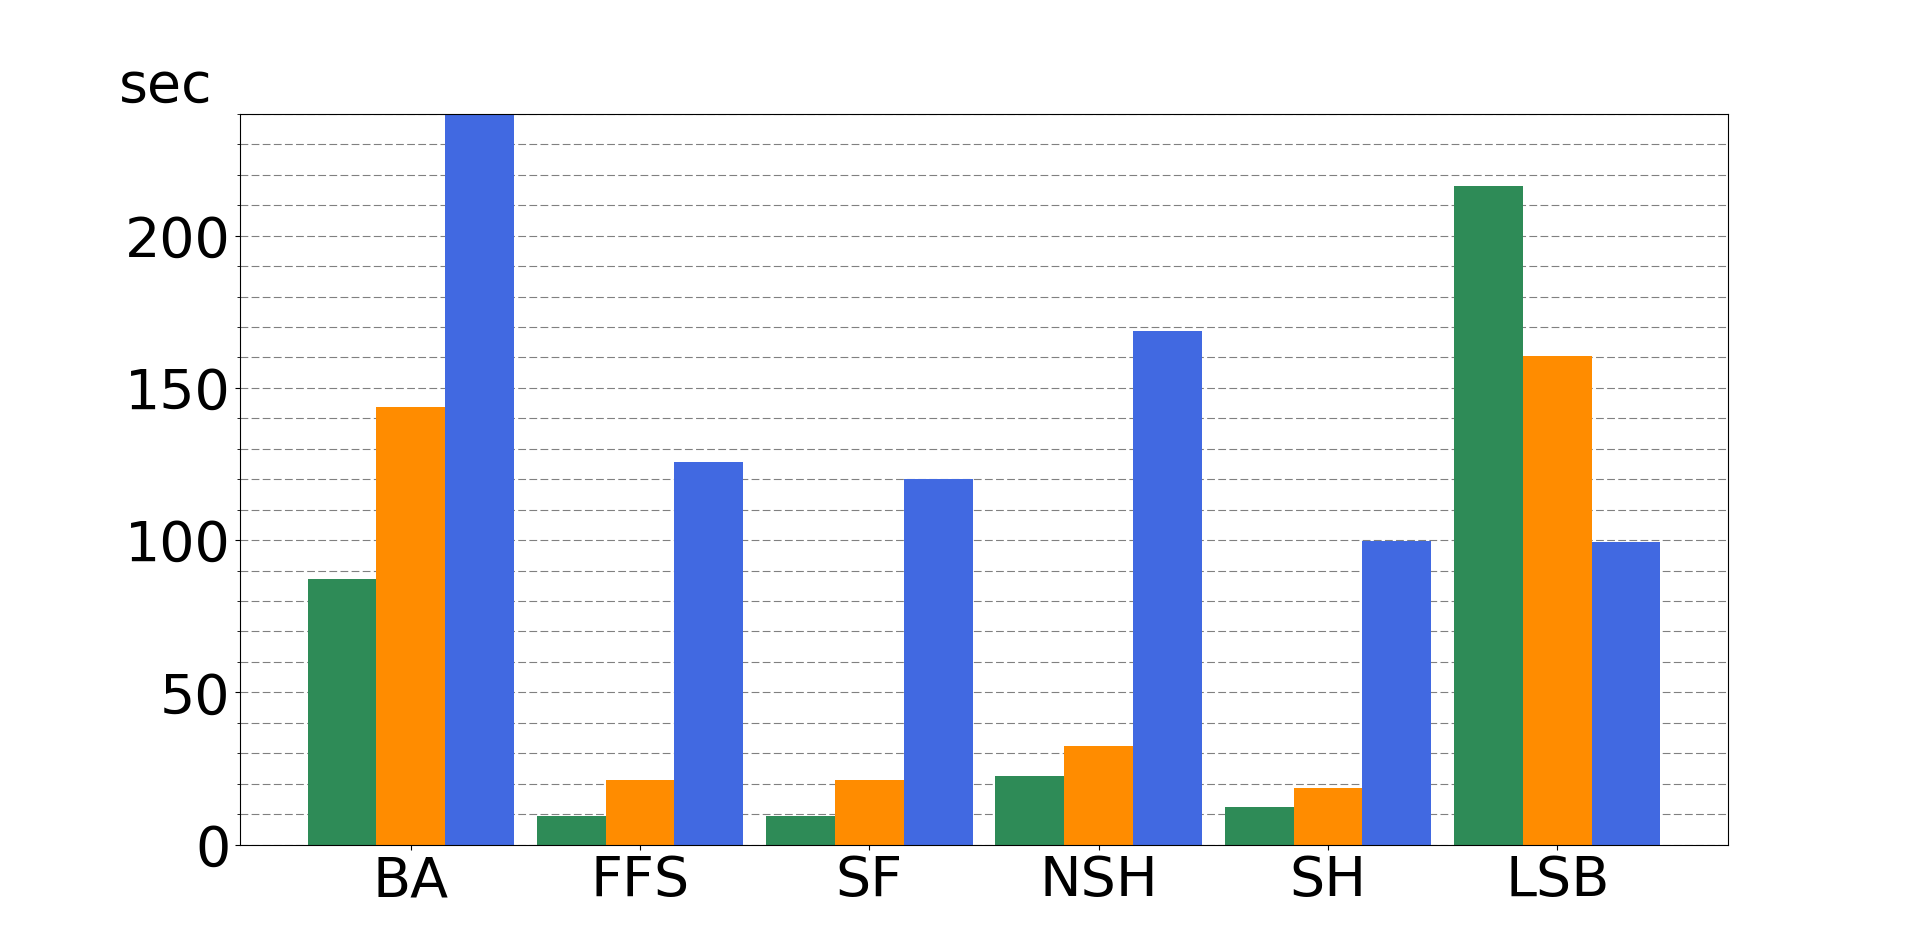
\includegraphics[width=\textwidth]{img/dens16}\caption*{Error = 16}}
\end{minipage}%
\begin{minipage}{.5\linewidth}
\centering
\subfloat{\label{dens:d}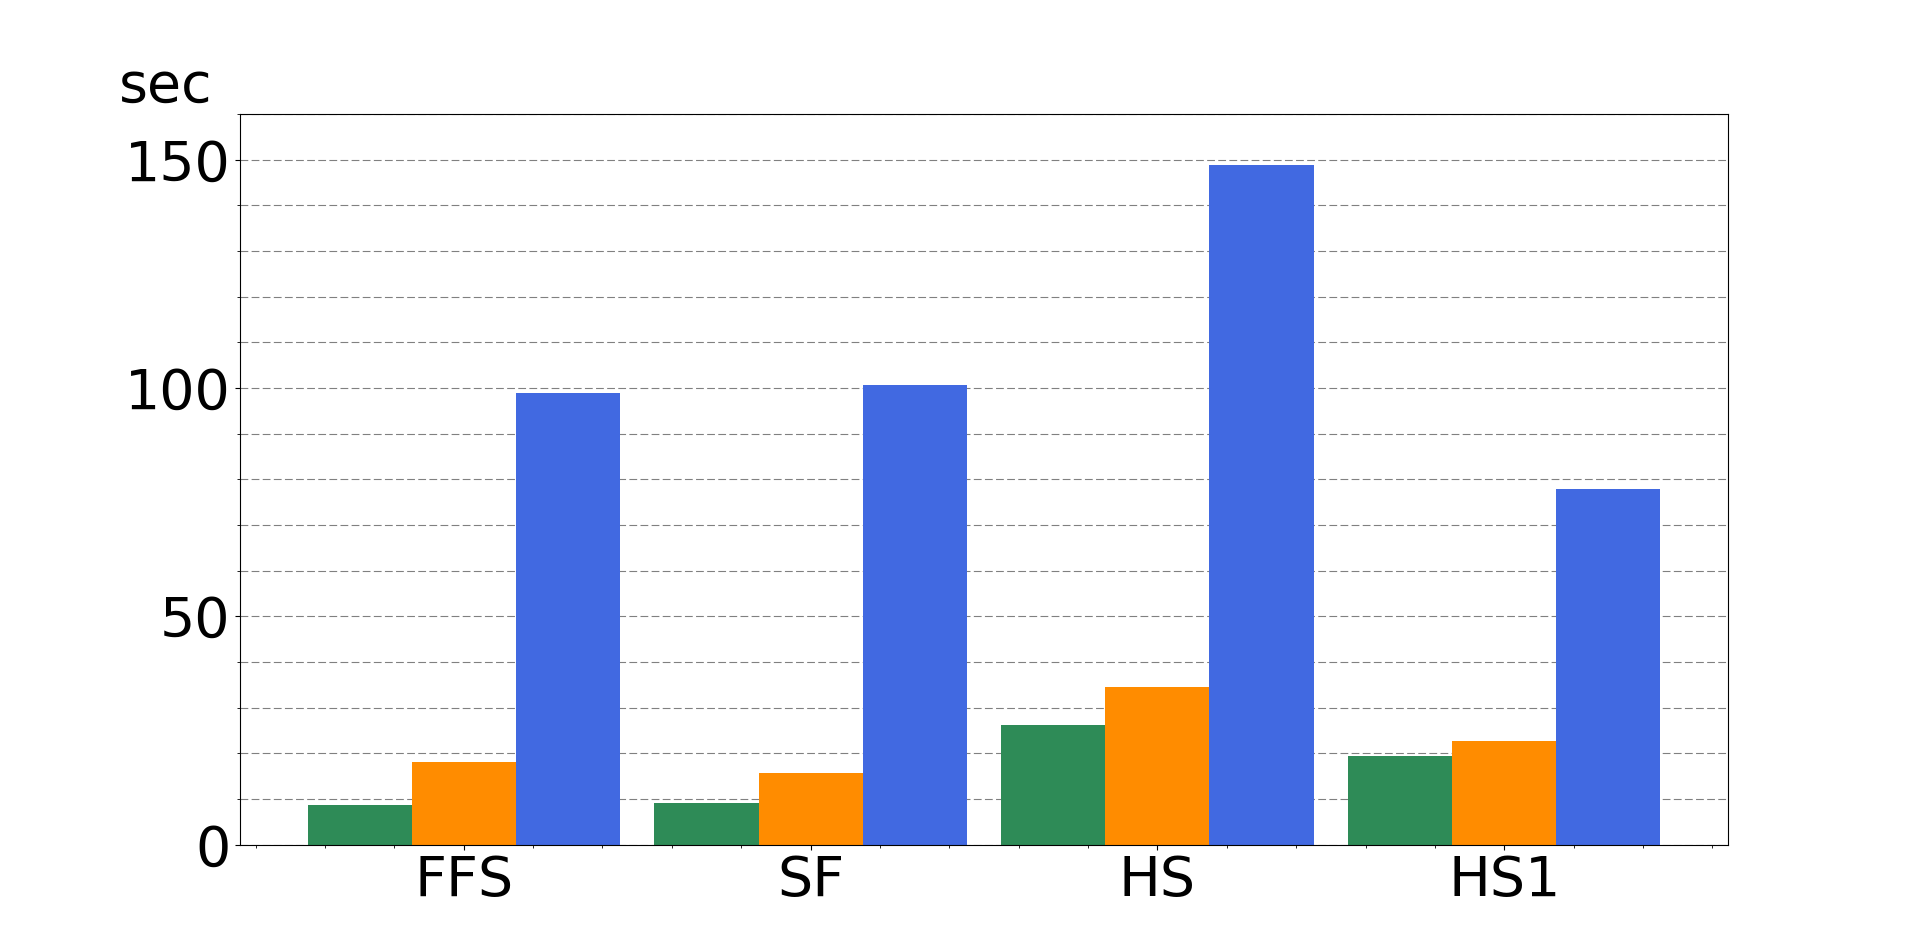
\includegraphics[width=\textwidth]{img/dens64}\caption*{Error = 64}}
\end{minipage}\par\medskip

\caption{Comparison on varying density of data}
\label{fig_densRes}
\end{figure}

\subsection{Dependency on dimensionality}
Three different files were used based on the number of dimensions which were: 2, 3 and 4. In the graph \ref{fig_dimRes} the green color belongs to the 2D file, orange is for the standard 3 dimensional file and blue shows 4 dimensions. It is clear that the bigger the number of dimensions the higher times. This happens because for more dimensions the algorithm gets into higher recursion levels than otherwise.

Second important thing to see in these graphs is that for low error rate and lower dimensionality hash algorithms are way worse than other non-brute solutions. This is caused by a high number of collisions and thus more expensive preverification. Because of the low data dimensionality there is only last dimension of data in the memory that will be hashed which means there is no reusage of already created hashes.

The higher the number of dimensions in chunks the better the reusage rate of hashing algorithms thus better scaling.

\begin{figure}
\begin{minipage}{.5\linewidth}
\centering
\subfloat{\label{dim:a}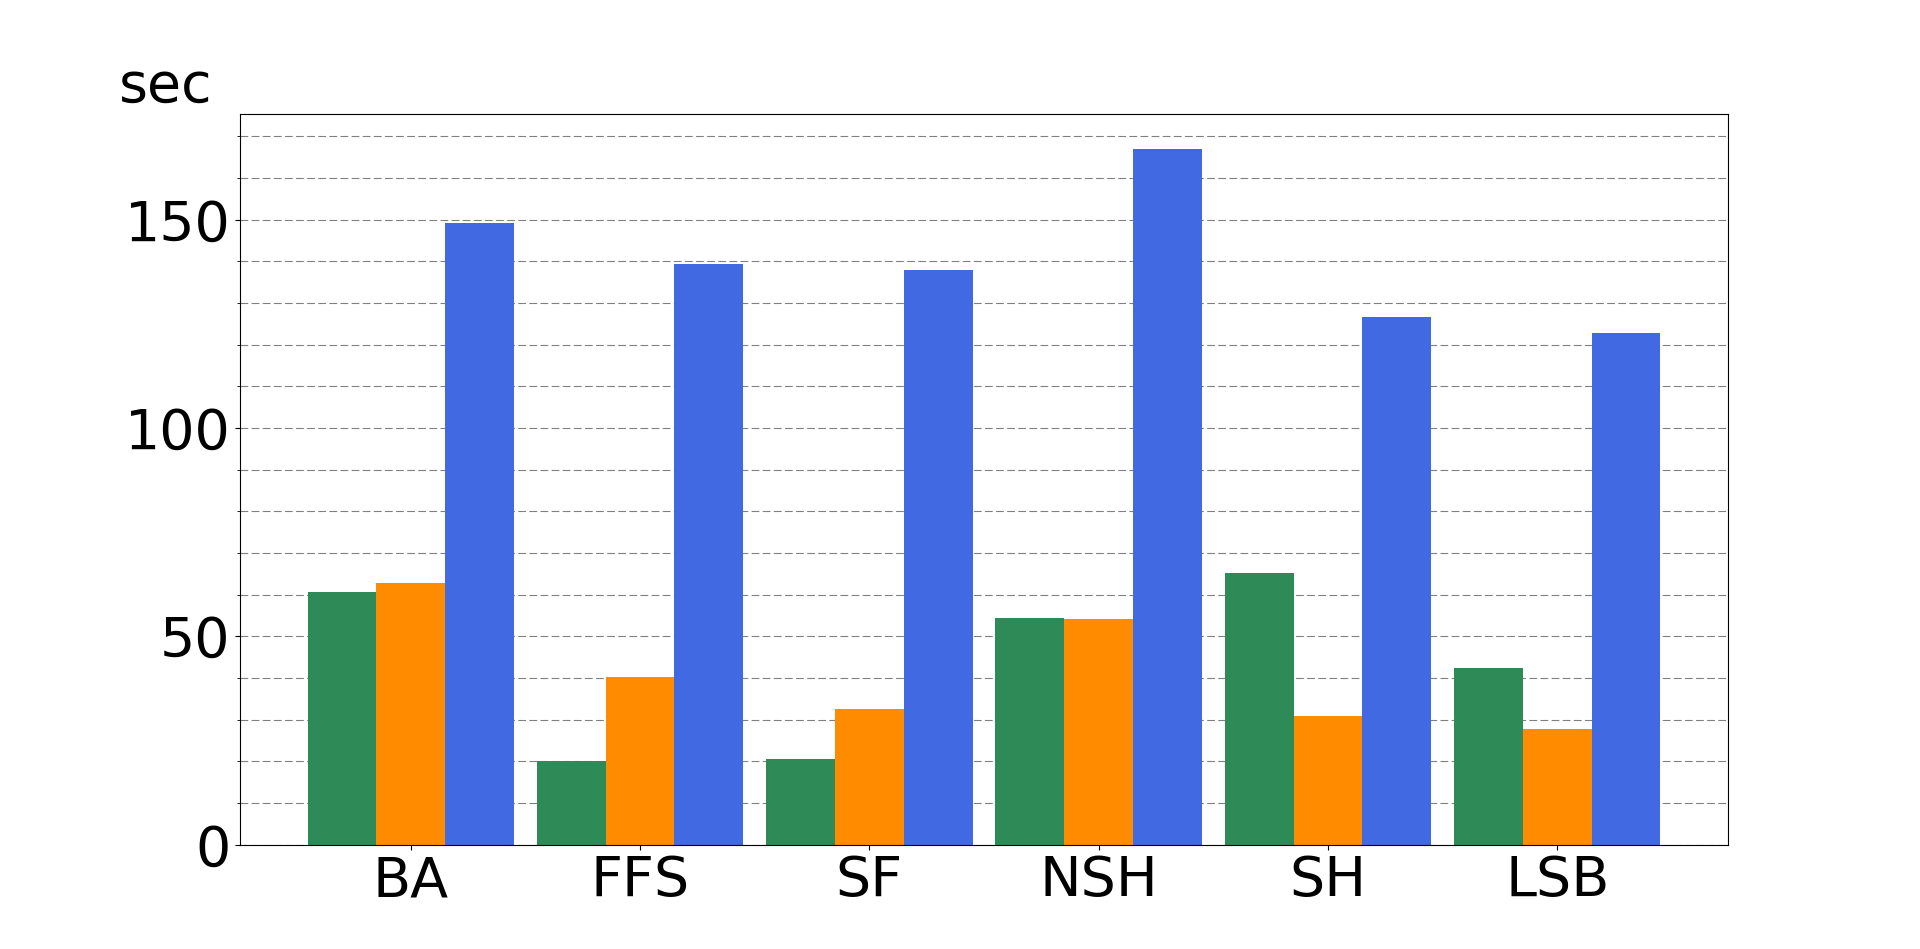
\includegraphics[width=\textwidth]{img/dim0}\caption*{Error = 0}}
\end{minipage}%
\begin{minipage}{.5\linewidth}
\centering
\subfloat{\label{dim:b}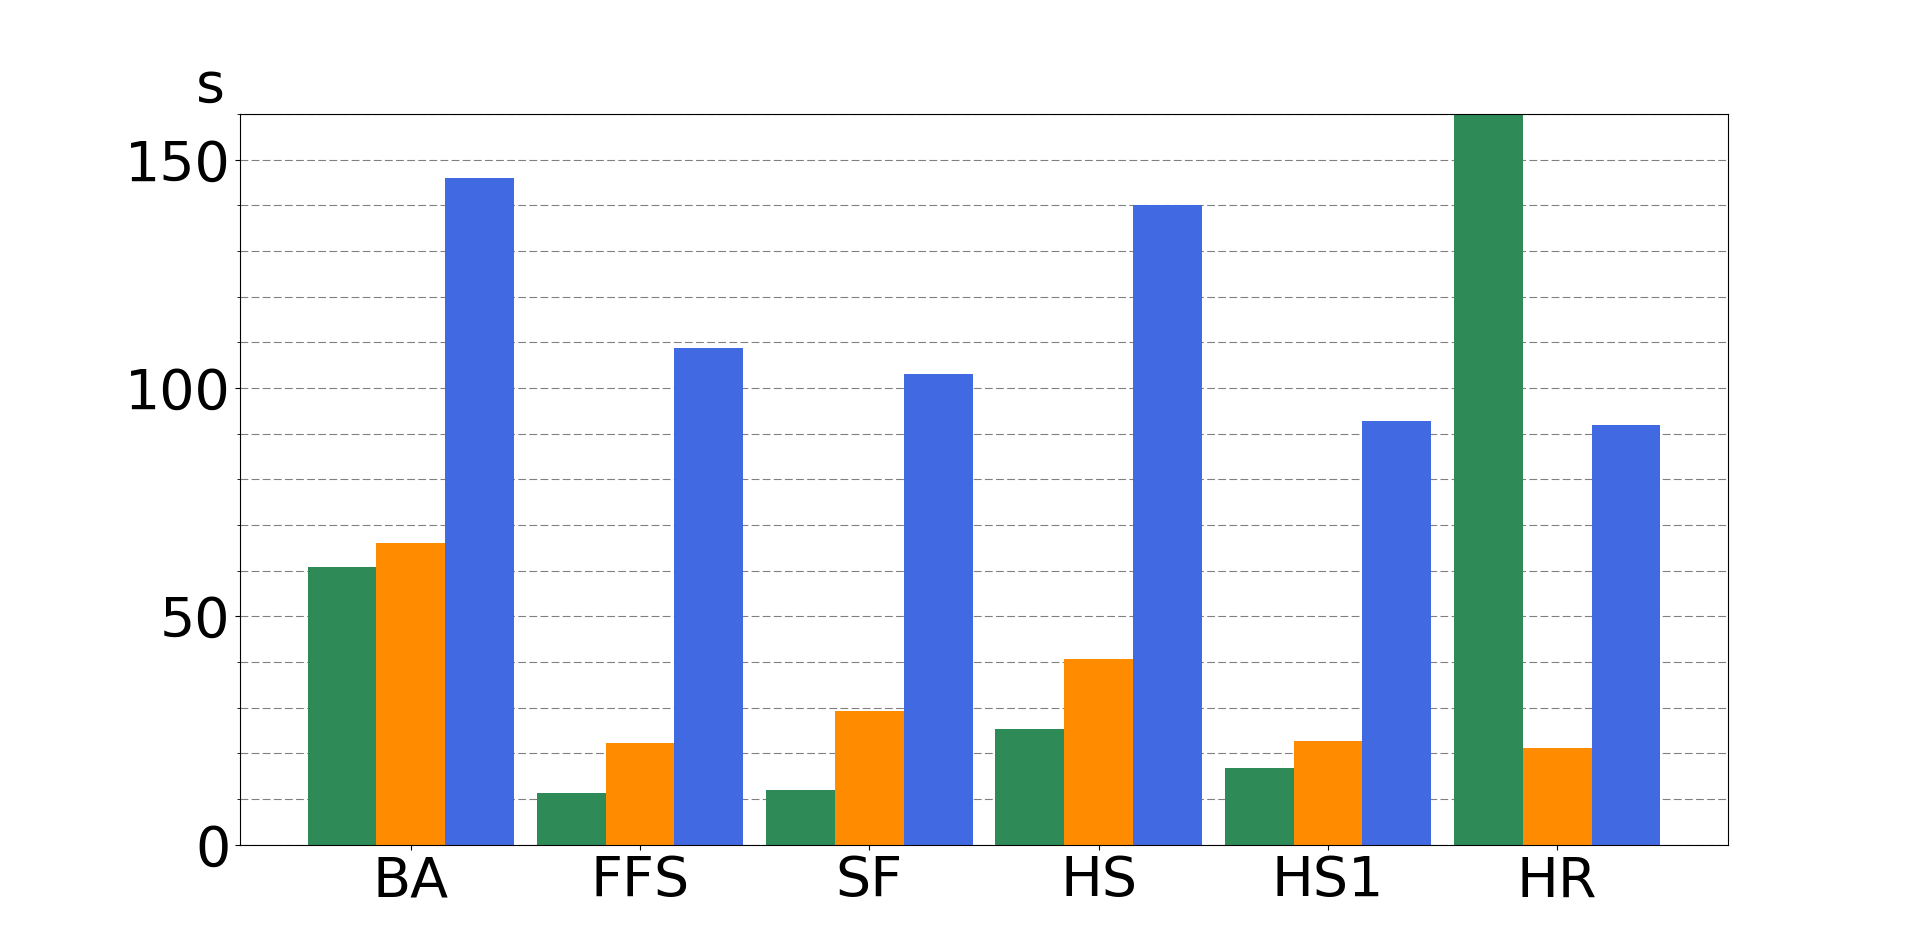
\includegraphics[width=\textwidth]{img/dim4}\caption*{Error = 4}}
\end{minipage}\par\medskip

\begin{minipage}{.5\linewidth}
\centering
\subfloat{\label{dim:c}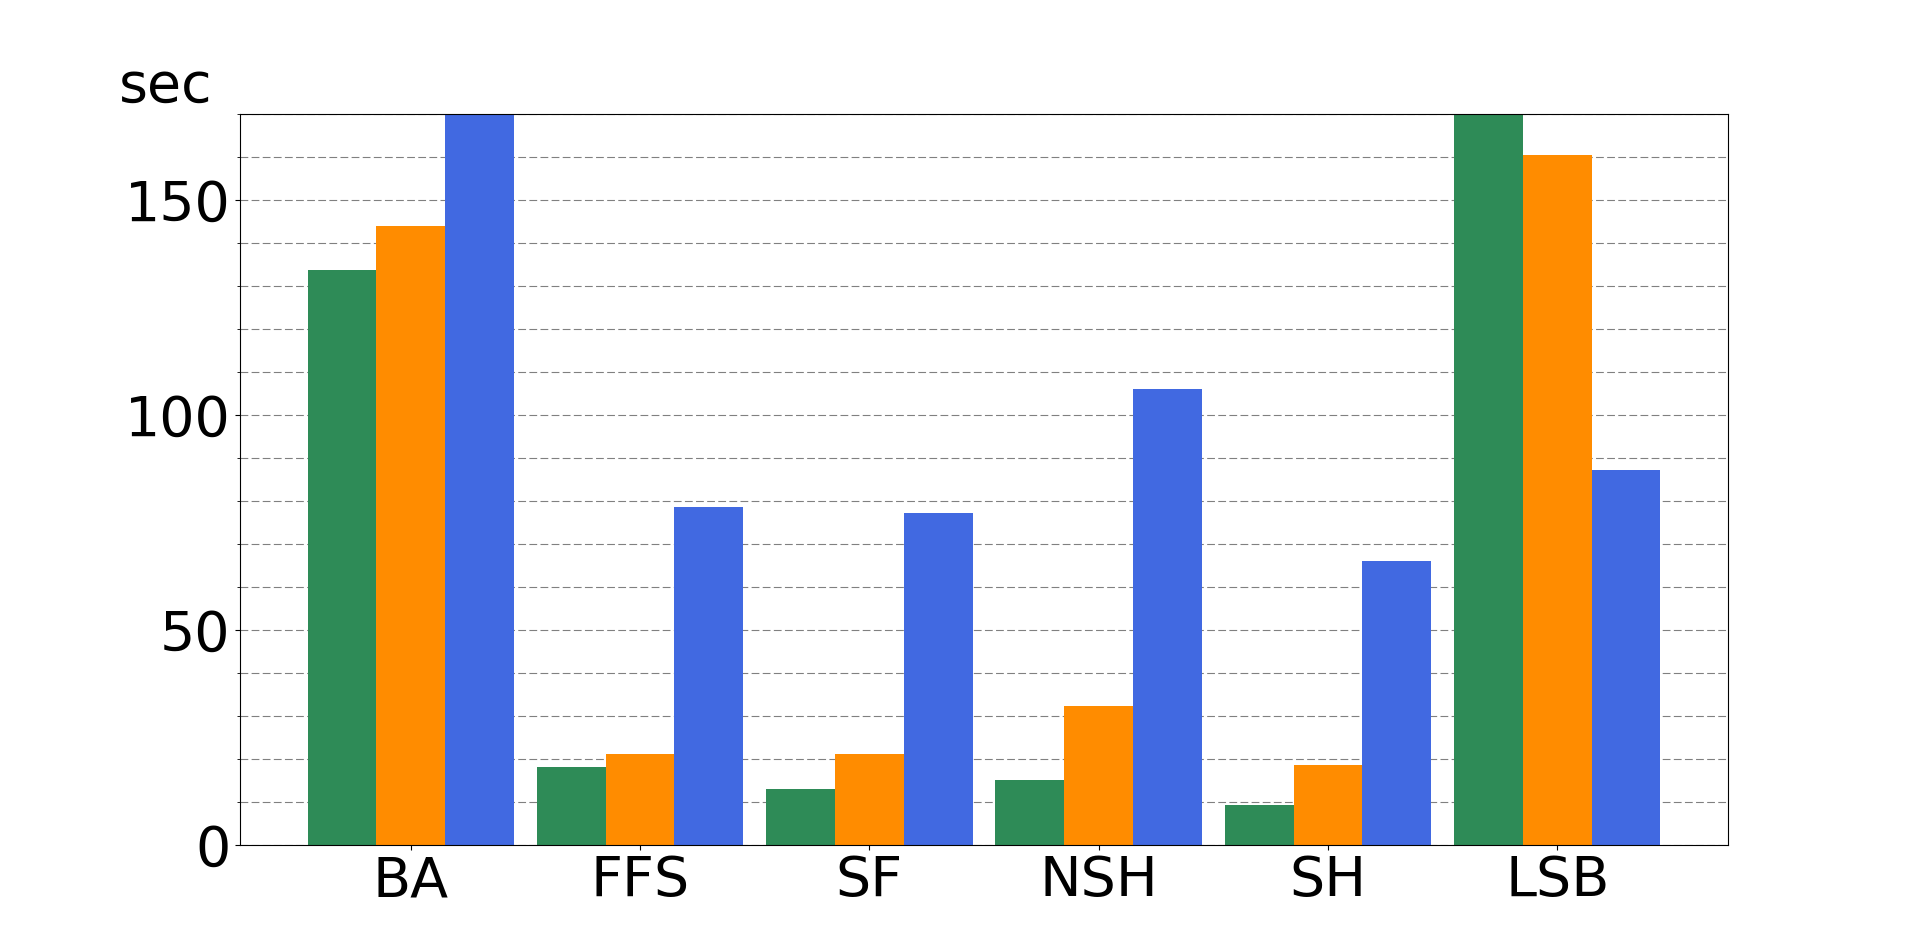
\includegraphics[width=\textwidth]{img/dim16}\caption*{Error = 16}}
\end{minipage}%
\begin{minipage}{.5\linewidth}
\centering
\subfloat{\label{dim:d}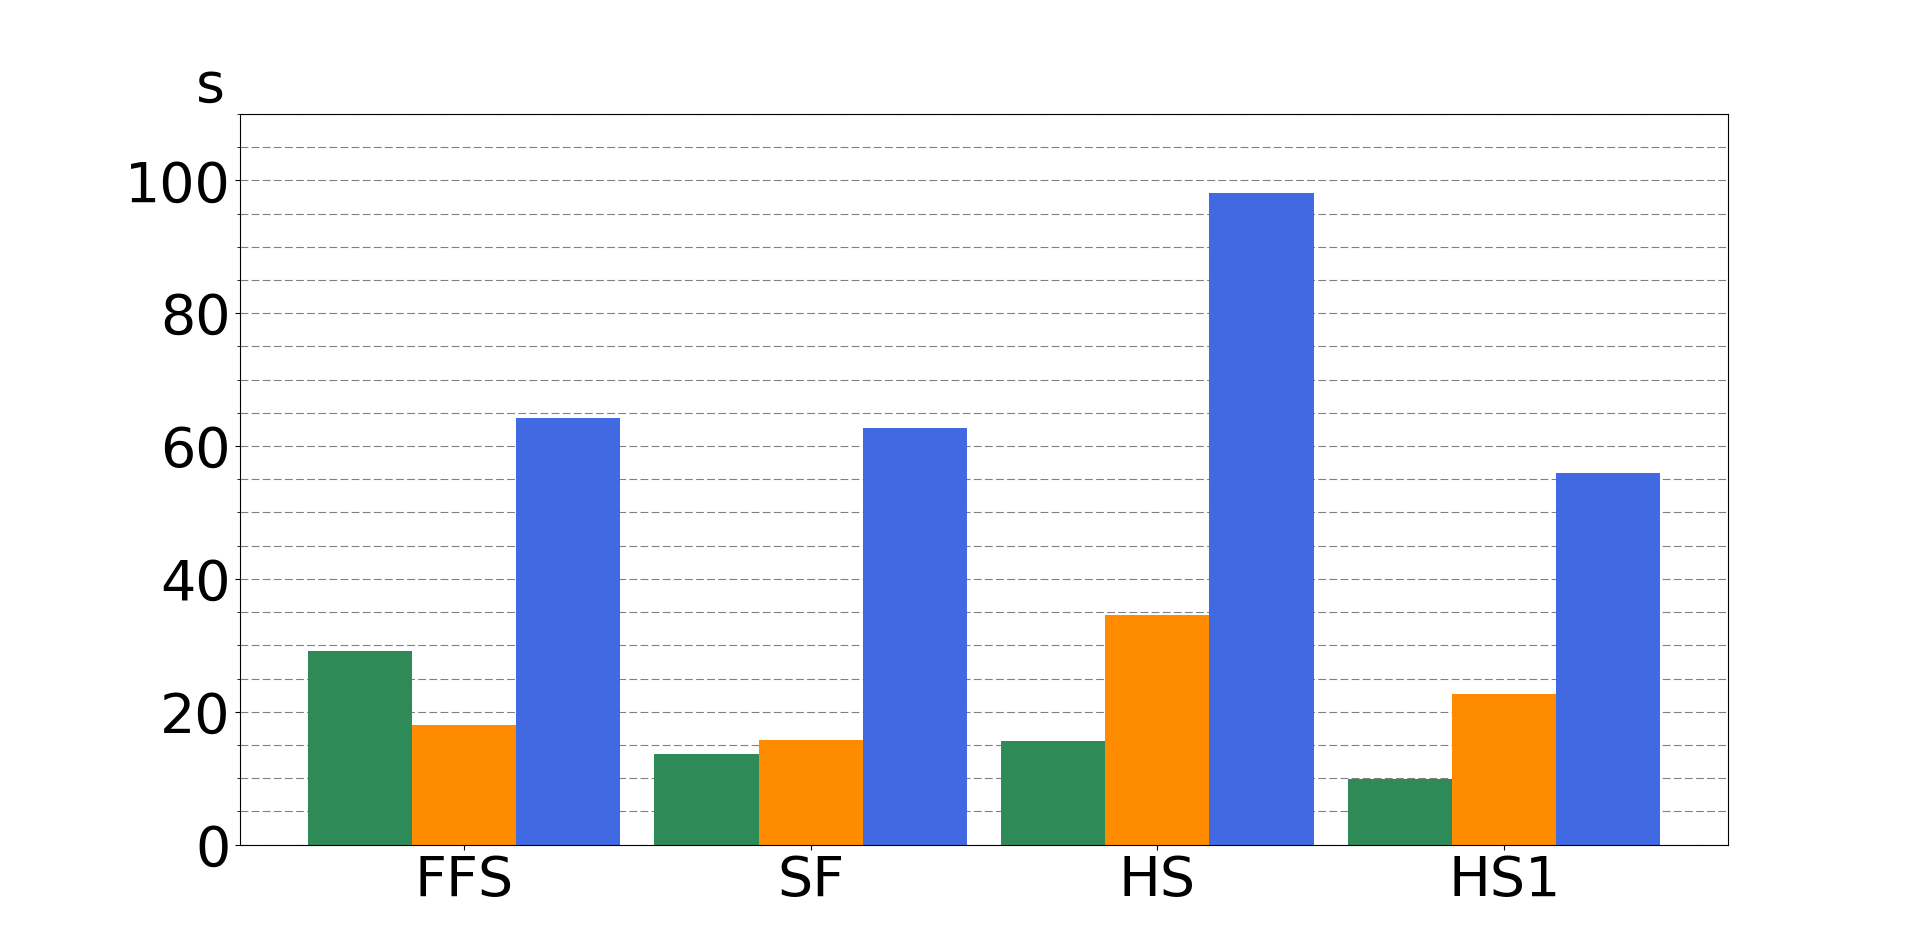
\includegraphics[width=\textwidth]{img/dim64}\caption*{Error = 64}}
\end{minipage}\par\medskip

\caption{Comparison on varying number of dimensions.}
\label{fig_dimRes}
\end{figure}

\subsection{Dependency on frequency of pattern occurrence}
Difference between input files were this time in the number of pattern occurrences. Standard file had the occurrence rate set to $0.1 \%$ while the other two had $1 \%$ and $0.01 \%$. In the figure \ref{fig_patRes} there can be seen only a slight difference in the times of comparing algorithms. This difference is caused only by the preverification step and dynamic checks as they need to control more possible solutions thus lasting longer.

On the other hand, there is nicely illustrated the difference between individual algorithms. 

Stricter Filter algorithm is always slightly better than FFS because preverification step is quicker than dynamic check. Also HS1 is always quicker than HS because there are no repeated hash constructions. Quality of HR is mainly in lower error rates.
%kdyz tam neni zobrazeny nic jinyho muzes se zminit, ze je dobre viditelne porovnani mezi jednolivejma algoritmama - a proc

\begin{figure}
\begin{minipage}{.5\linewidth}
\centering
\subfloat{\label{pat:a}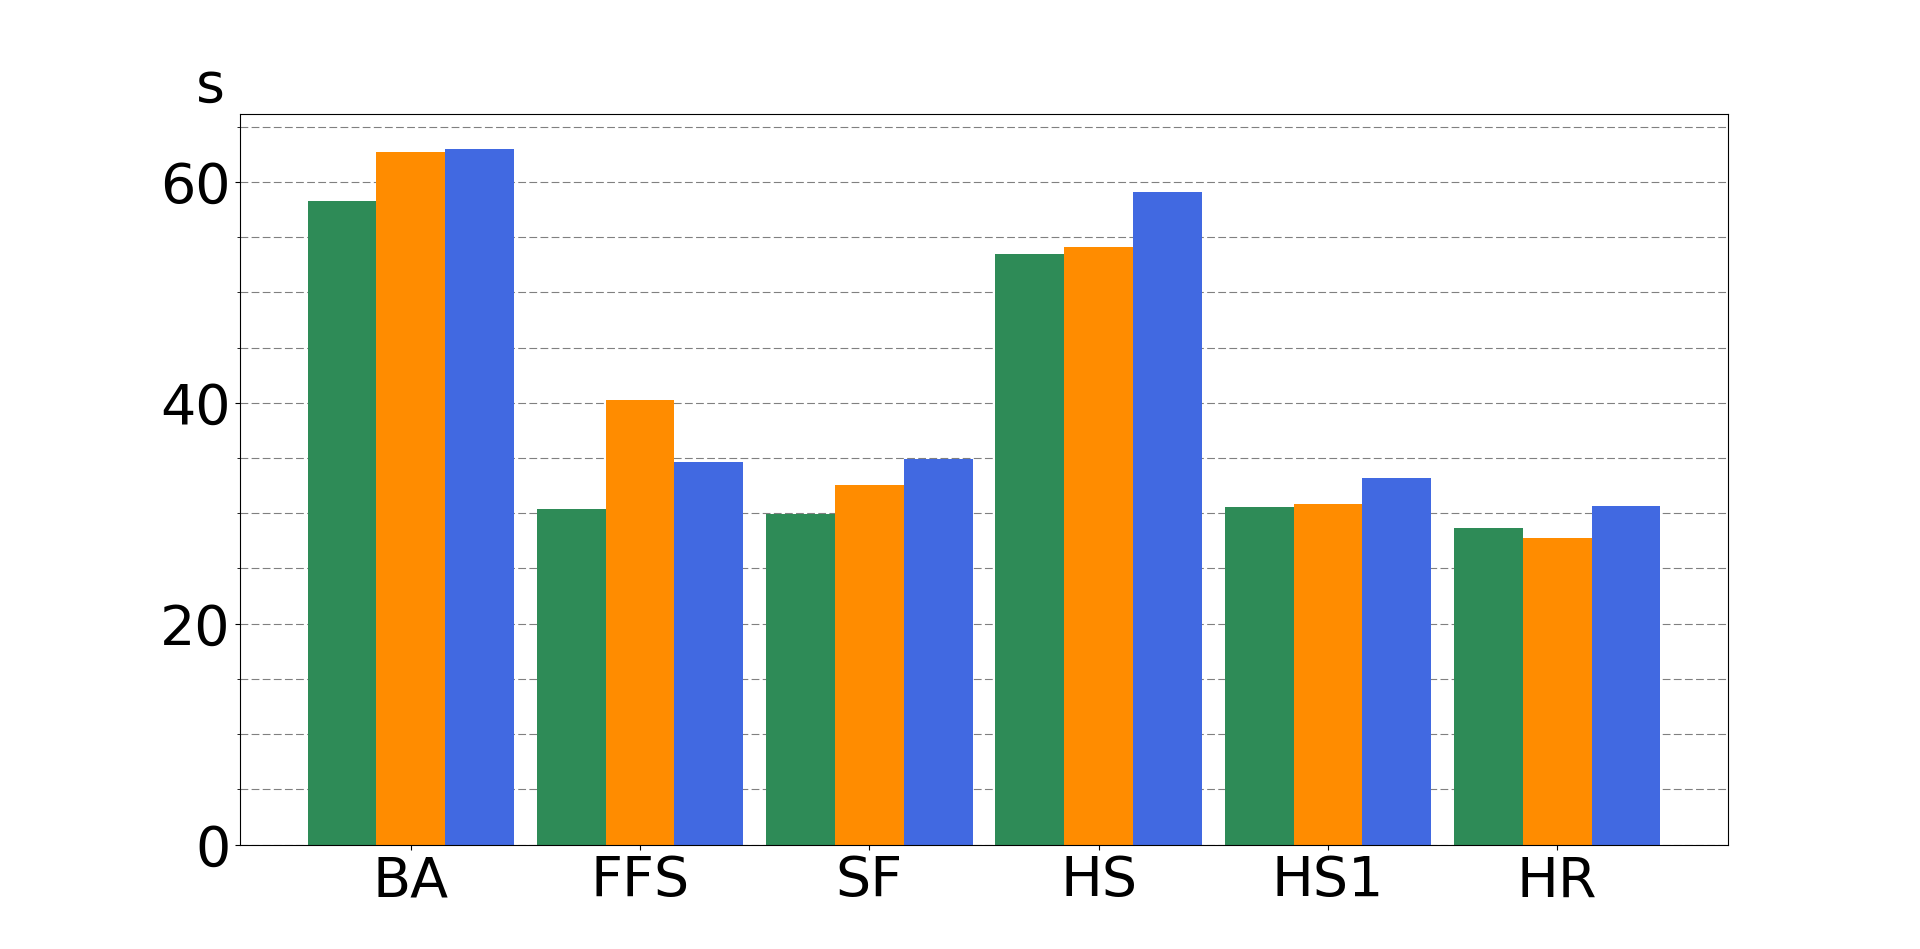
\includegraphics[width=\textwidth]{img/pat0}\caption*{Error = 0}}
\end{minipage}%
\begin{minipage}{.5\linewidth}
\centering
\subfloat{\label{pat:b}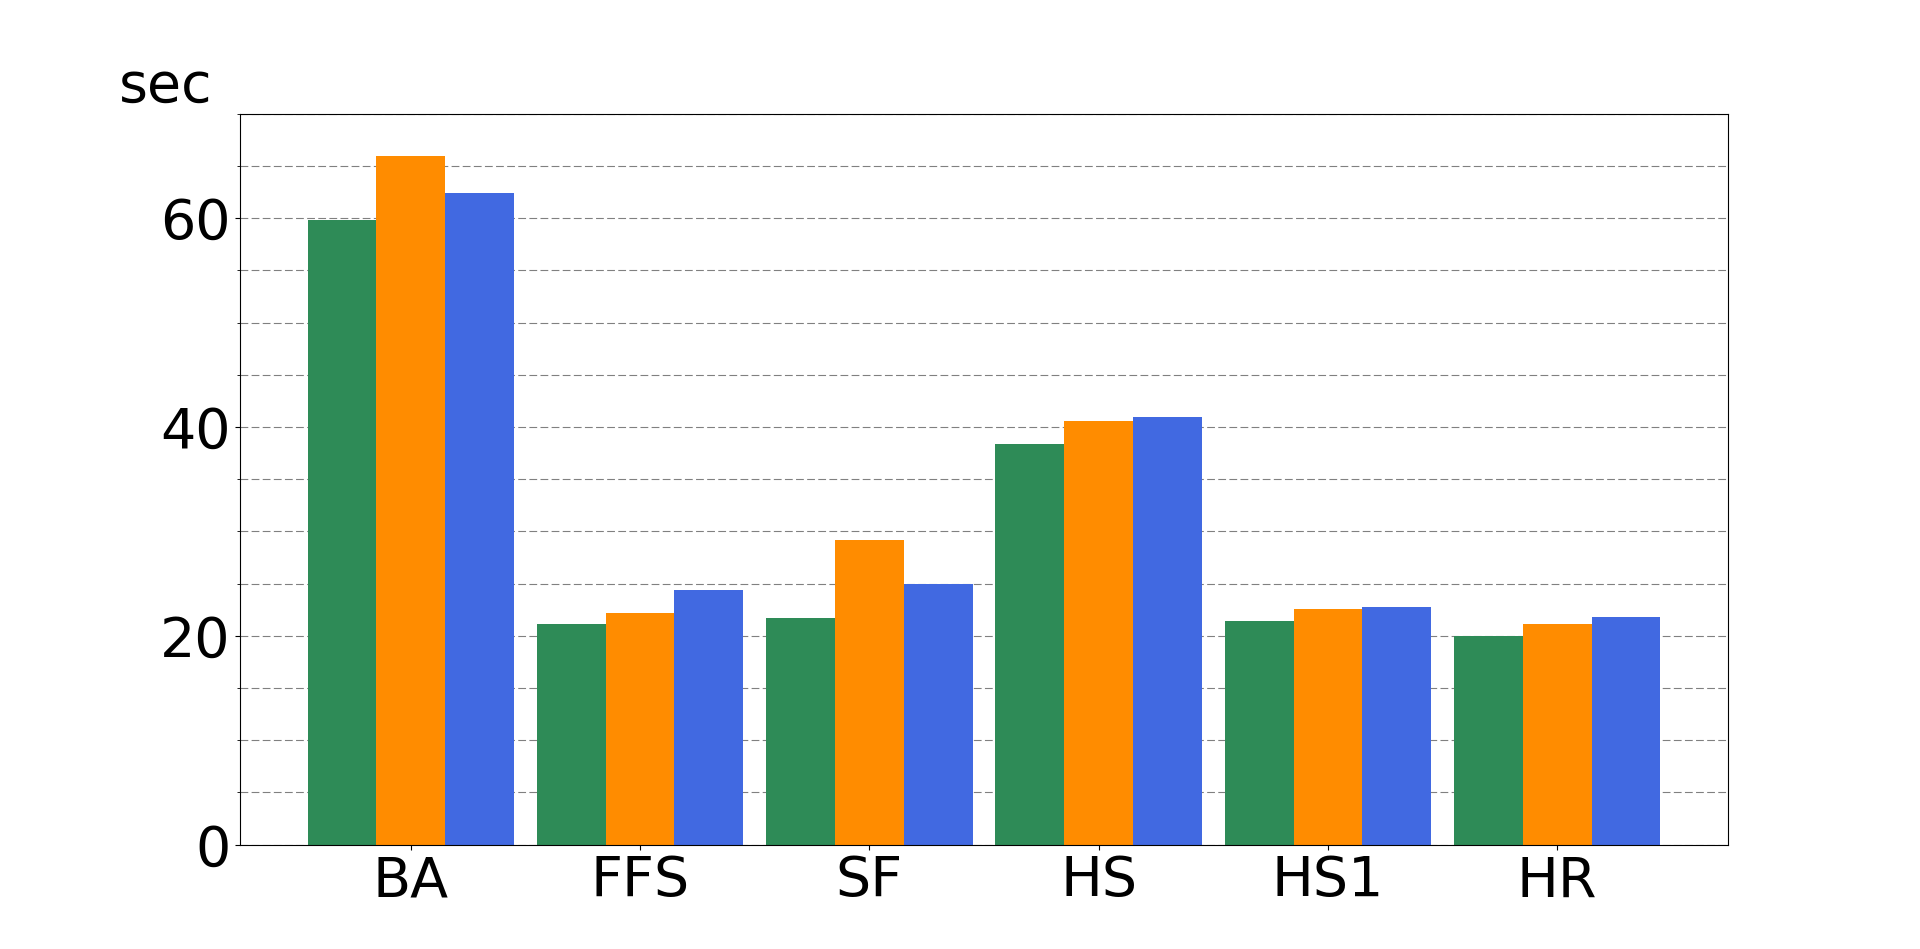
\includegraphics[width=\textwidth]{img/pat4}\caption*{Error = 4}}
\end{minipage}\par\medskip

\begin{minipage}{.5\linewidth}
\centering
\subfloat{\label{pat:c}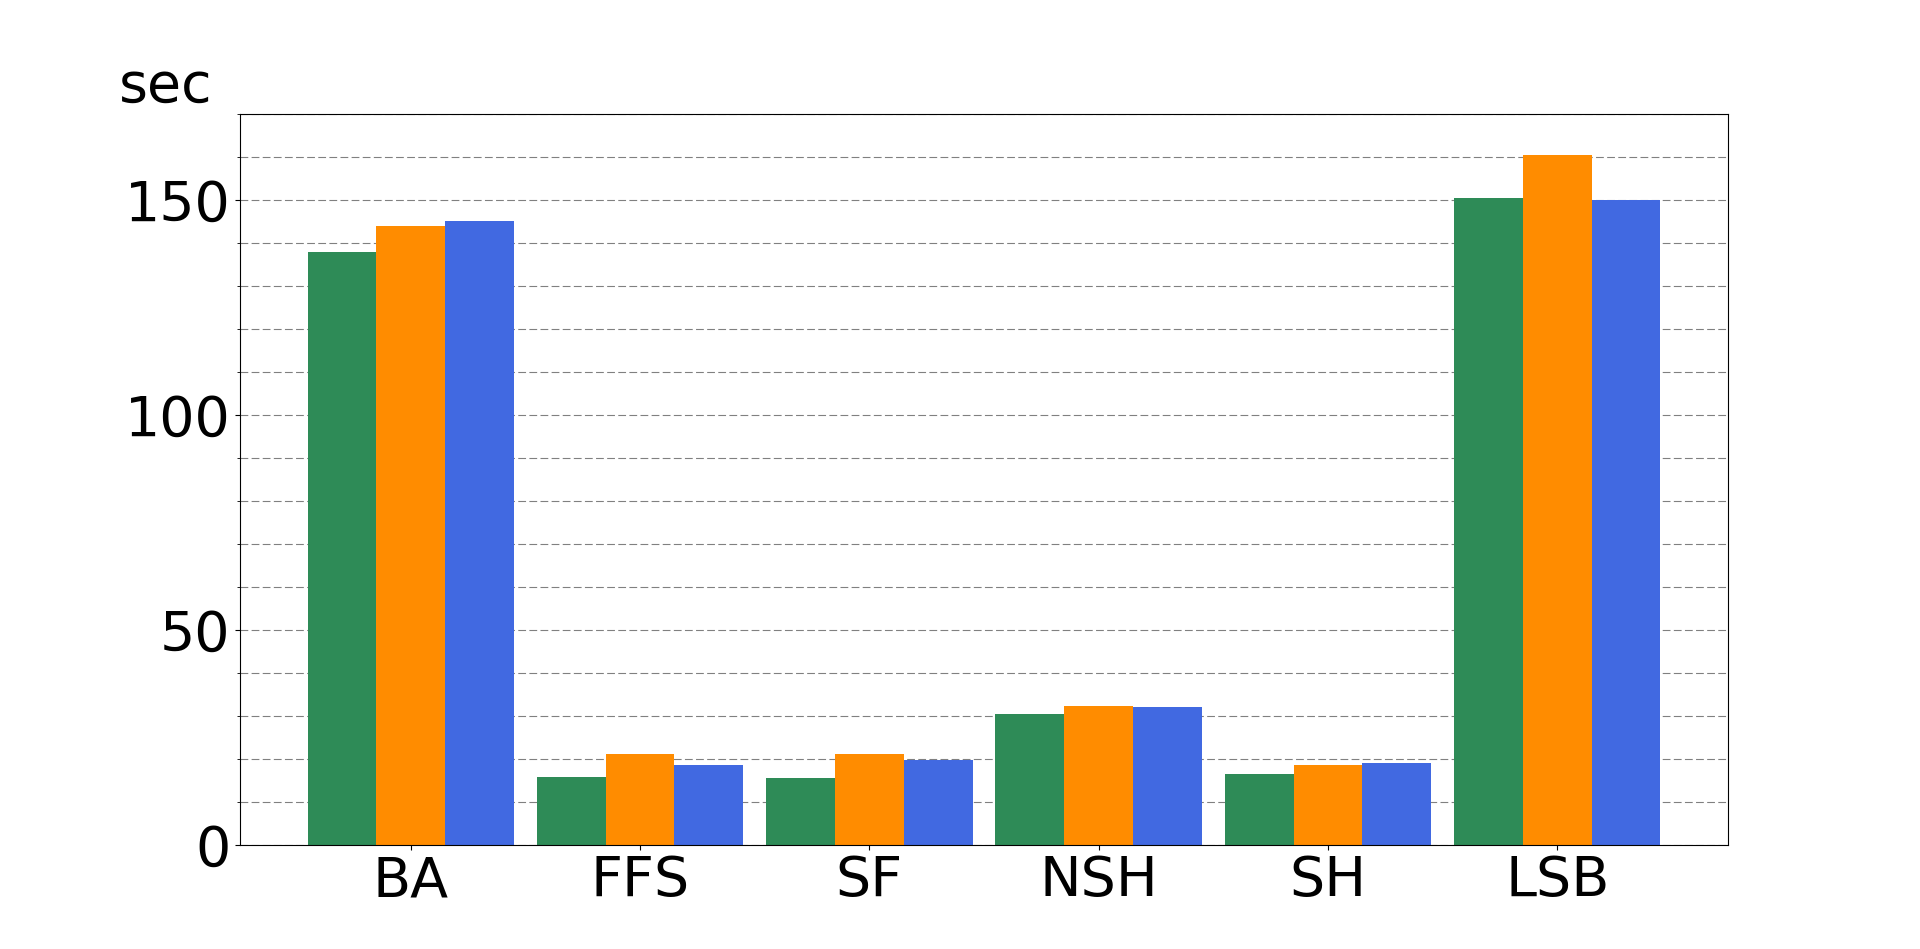
\includegraphics[width=\textwidth]{img/pat16}\caption*{Error = 16}}
\end{minipage}%
\begin{minipage}{.5\linewidth}
\centering
\subfloat{\label{pat:d}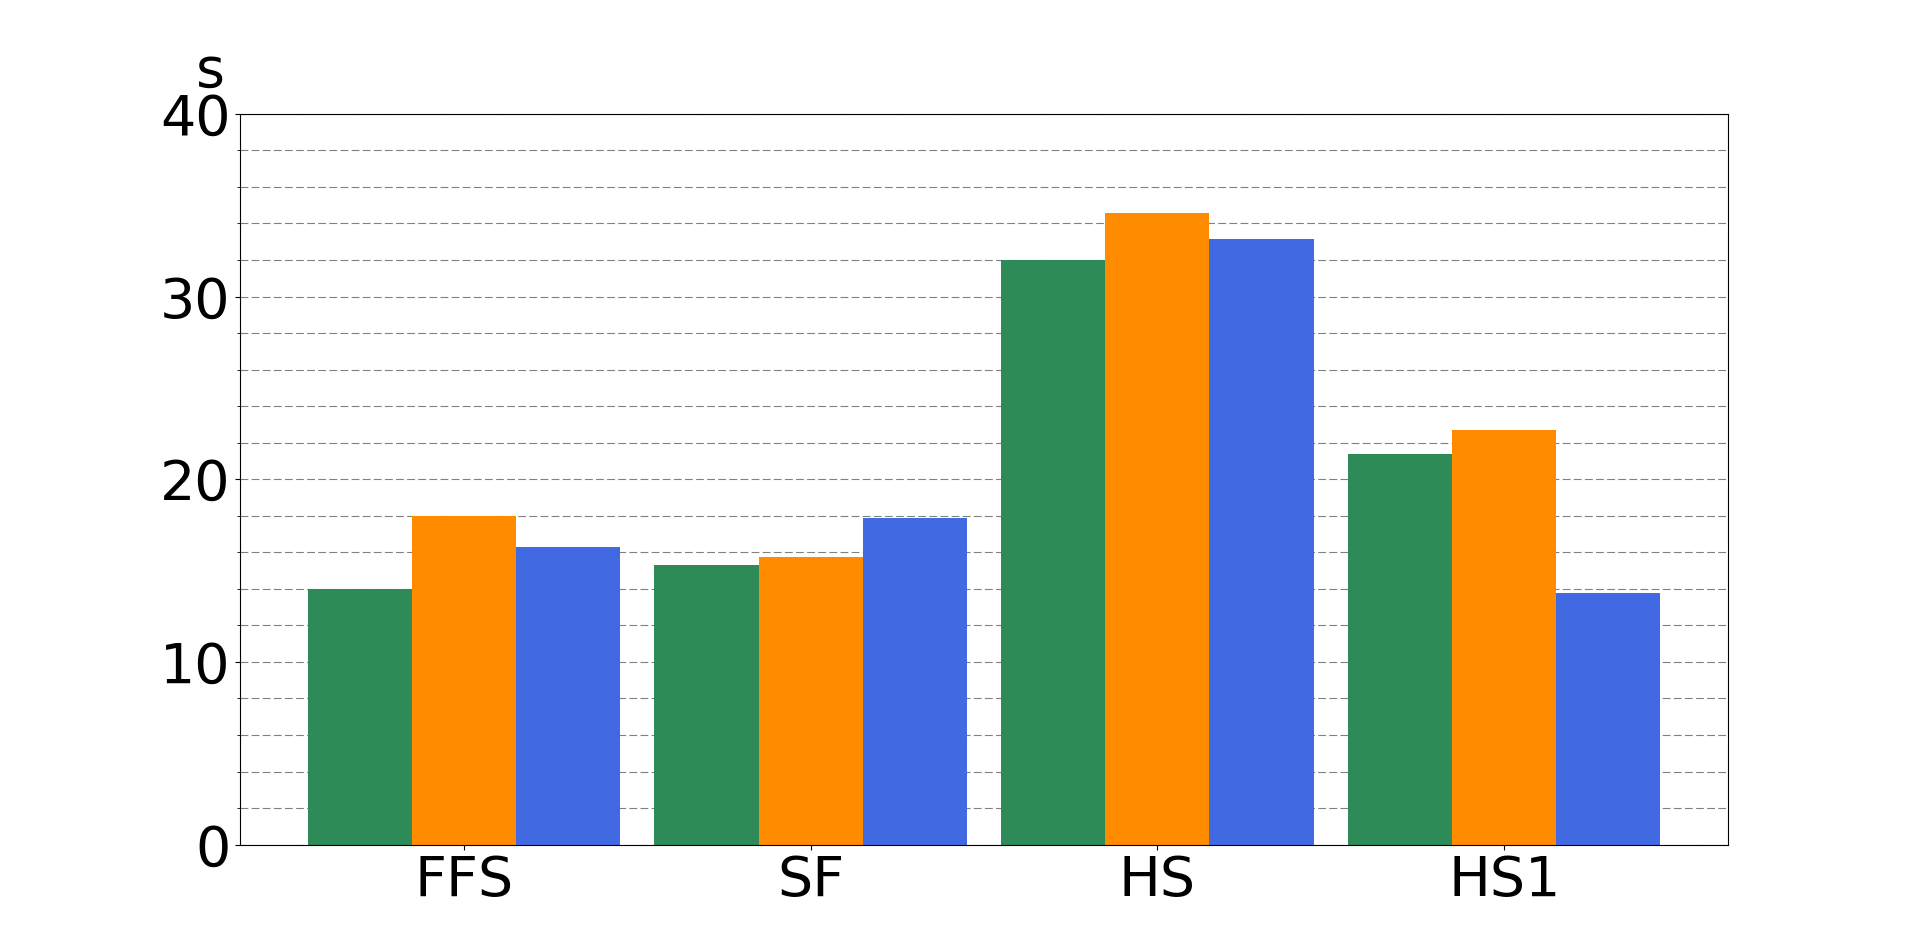
\includegraphics[width=\textwidth]{img/pat64}\caption*{Error = 64}}
\end{minipage}\par\medskip

\caption{Comparison using varying frequency of pattern occurrence.}
\label{fig_patRes}
\end{figure}

\subsection{Dependency on input file size}
In the last graph figure \ref{fig_sizeRes} there can be seen comparison of standard (orange) file and file of the size 4 GB but measured twice, first with the pattern of size $64\times64\times64$ and second with the standard pattern (size $16\times16\times16$).
% a proc patern 64 a 16? - 16 protoze standard a 64 aby to bylo podobnejsi pomerem
% taky ze tam je logaritmicky meritko, aby to bylo lip videt

The difference in the pattern size proved to have only a slight effect on the final reached times. It is no surprise that the times are different. %co to je za zblept? to je snad jasny ze to bude vetsi, ale jestli to je spravne vetsi


\begin{figure}
\begin{minipage}{.5\linewidth}
\centering
\subfloat{\label{size:a}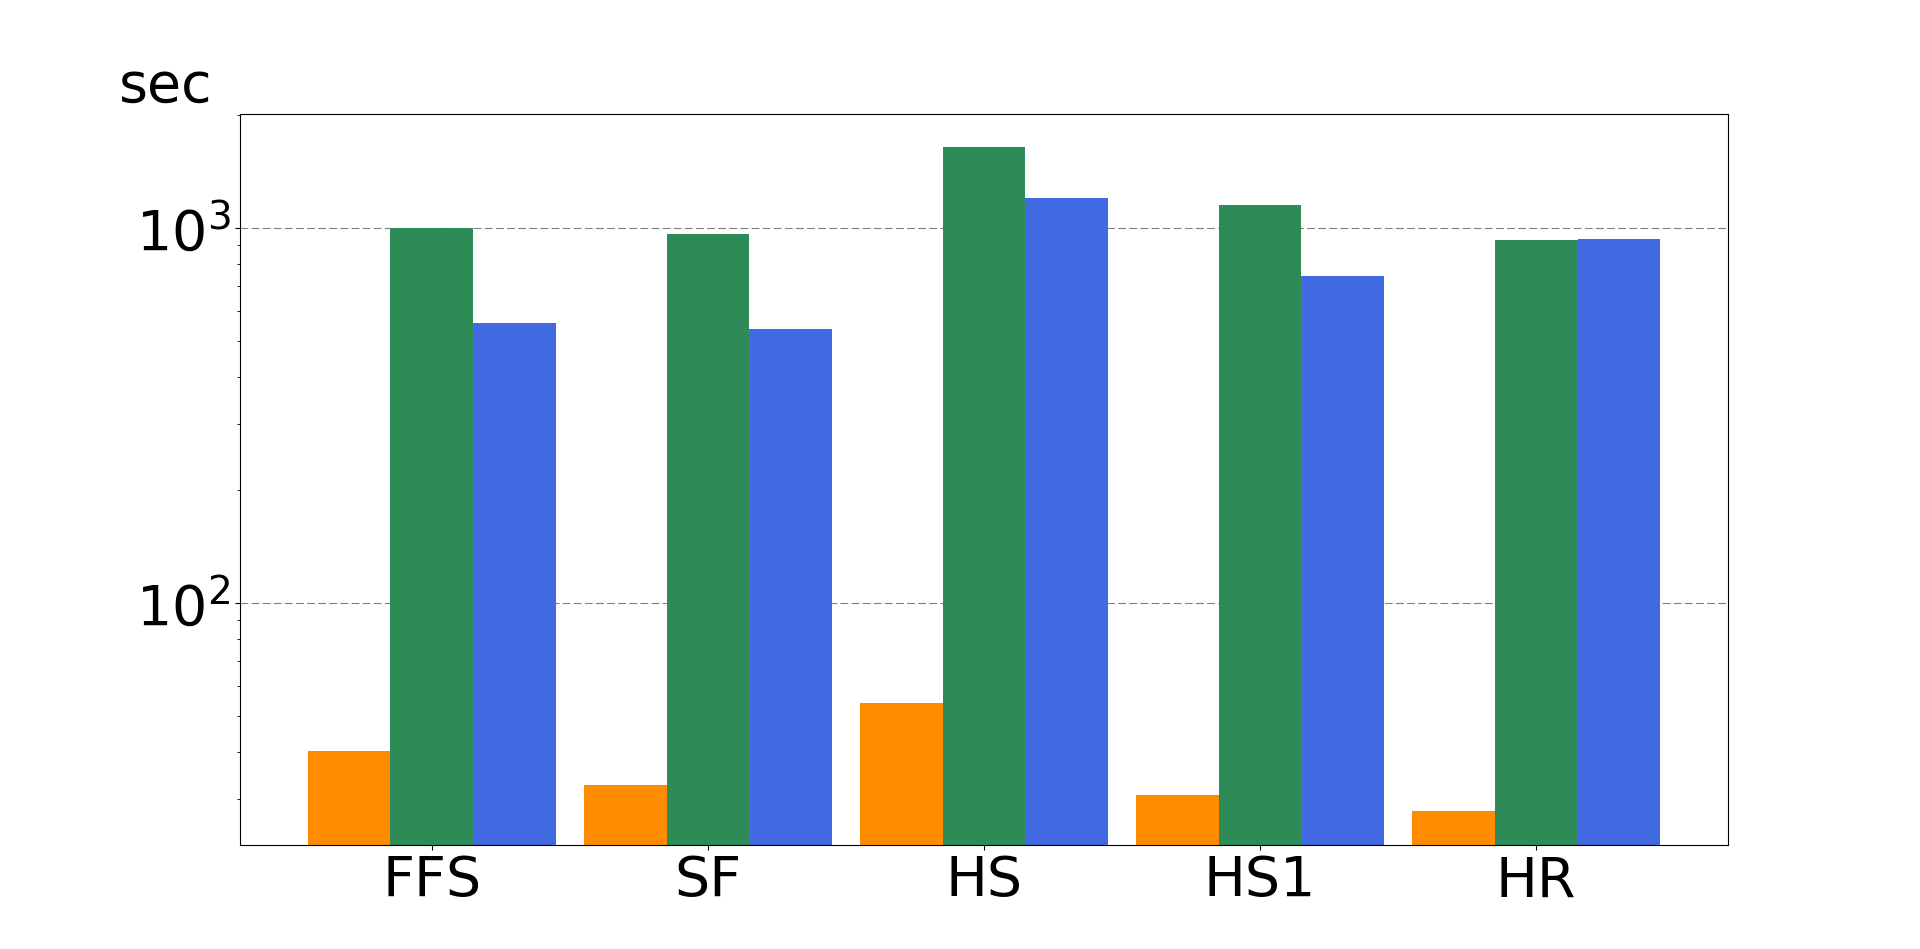
\includegraphics[width=\textwidth]{img/size0}\caption*{Error = 0}}
\end{minipage}%
\begin{minipage}{.5\linewidth}
\centering
\subfloat{\label{size:b}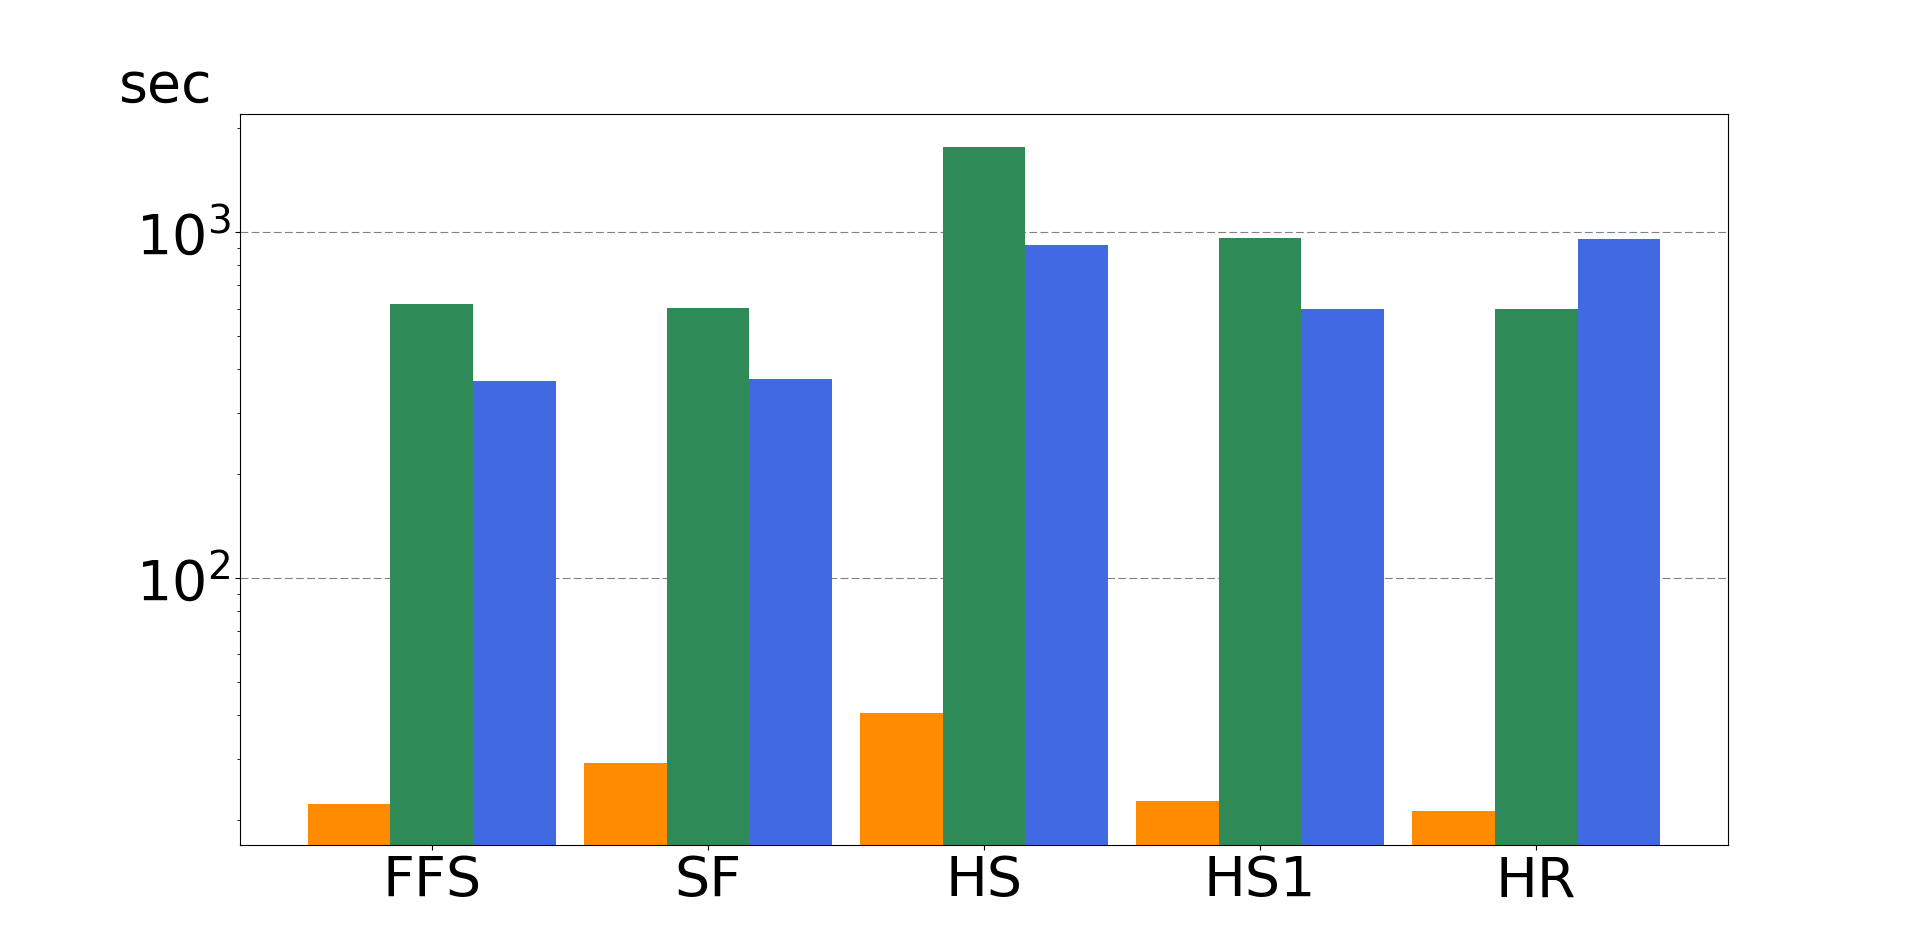
\includegraphics[width=\textwidth]{img/size4}\caption*{Error = 4}}
\end{minipage}\par\medskip

\begin{minipage}{.5\linewidth}
\centering
\subfloat{\label{size:c}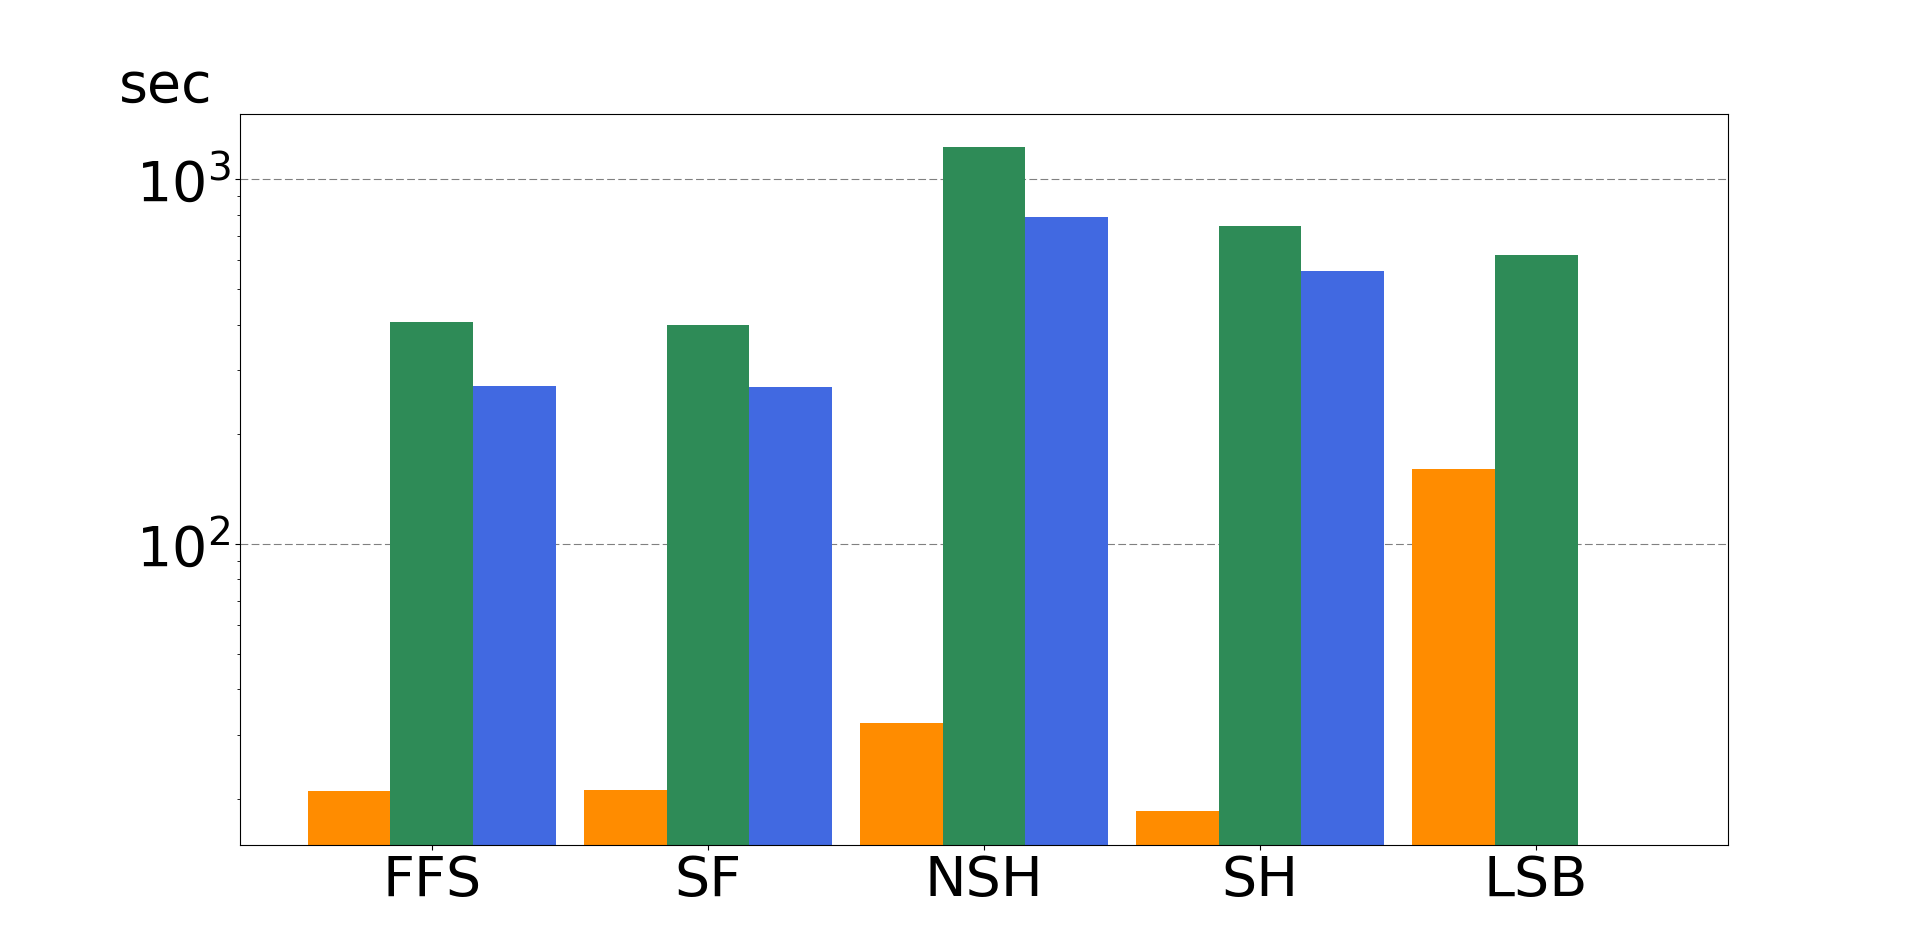
\includegraphics[width=\textwidth]{img/size16}\caption*{Error = 16}}
\end{minipage}%
\begin{minipage}{.5\linewidth}
\centering
\subfloat{\label{size:d}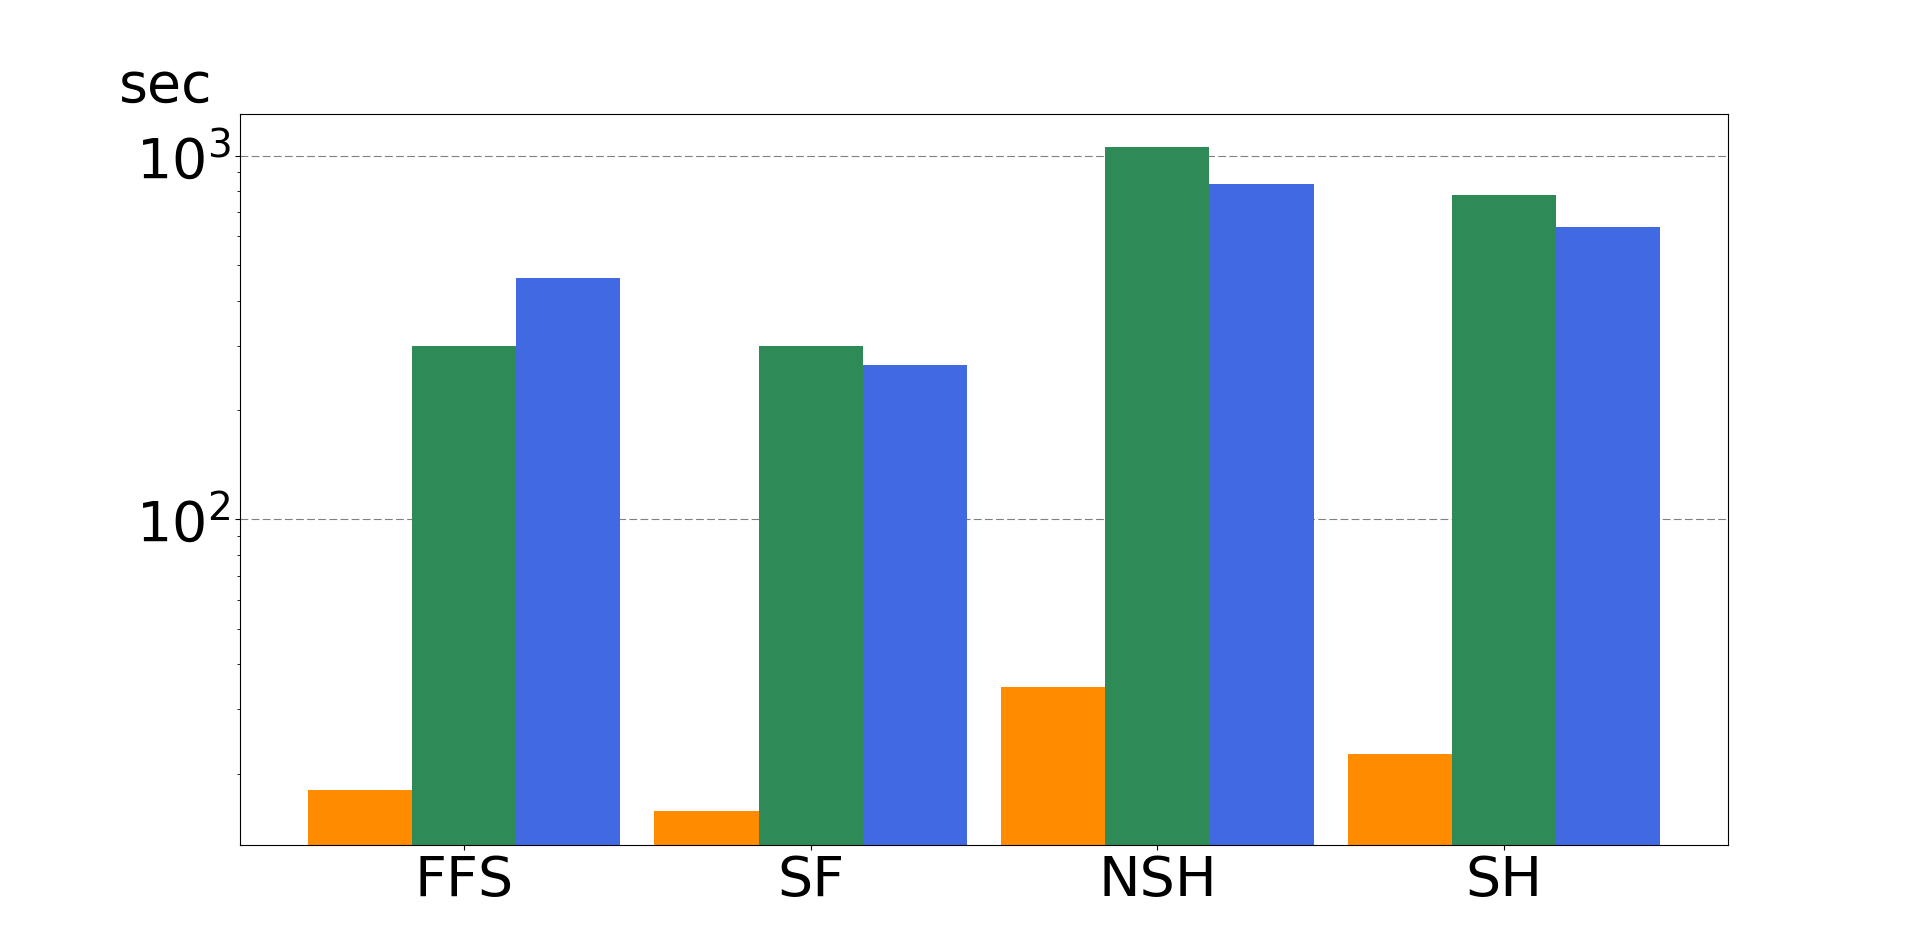
\includegraphics[width=\textwidth]{img/size64}\caption*{Error = 64}}
\end{minipage}\par\medskip

\caption{Test on 4GB data file.}
\label{fig_sizeRes}
\end{figure}


\subsection{Dependency on error rate}
In all the figures mentioned in previous sections, there can be seen that the higher the error rate the higher the times. This is caused by the course of action of all algorithms used, i.e. they all need to control more data before the maximum number of errors is found. % to plati jen u app brutu...ostatni hledaji identitu a pak se to jen preverifikuje...spis napis treba pocty tech prednalezenejch reseni...ze hash tim trpi ale co to ma zas za vyhody

This is much more obvious when looking only at the hash algorithms, which with the increasing error rate have multiple times higher collision rate and that makes them much worse than Stricter Filter and Fast Filter for high number of errors. However, when approached with low error rate and low density of data they prove to be better solution than Navaro and Baeza-Yates algorithms.
%z jakyho duvodu? (part size - hlavne u rolling hashe) - moznost zmenit pocitani j aby to bralo v uvahu hashovani a nepouzivalo moc maly part sizy

\section{Memory usage}
Implemented solutions uses a cache like memory system with the size of $max(64, m)$ where $m$ is the size of the pattern. This means that when the requested file is not in the memory it will be loaded into cache and if the cache is full the oldest data are discarded. 

When taking brute solution as a base line that uses only cache and pattern memory, FFS and SF algorithms do not use any added memory except for dynamic check that needs only extra space for creating of matrix of size $m\times m$ for the alignment purposes. Algorithms using hashes need extra space for the hashed pattern but the rest of its memory usage is the same as in the SF algorithm because the memory needed in each dimension is $\lceil 2\times n\rceil$ and thus the memory usage is very similar. % tohle nedava moc smysl...proste tam napis ze to zabere radove stejne, a jen ani ne 2krat tolik, protoze se ty hashe ulozi do podobny struktury jako normalni data, jen diky tomu ze to jsou hashe tak je to mensi
%navic vlastne ten prvni hash alg pouziva extra pamet jen na pattern, to tam taky napis

\subsection{Binary chunking}
In the table \ref{tab_chunk} there can be seen how using the binary format affects the size of the used data files. There can be seen that usage of the chunking lowers the size of the file about at least $60 \%$. This is because all the data values fits into 2 bytes and there is no need to store information about the dimensions as it is in the name of the file. 
%there can be seen zni divne a obzvlast 2krat za sebou
%60% je nesmysl..to ze mas zrovna cisla na 60% neznamena ze je to 60% --proste to snizuje o hodne, ale ze to dosta zavisi na densite...kdybys mela dostatecne malou density (promile treba) tak to bude i horsi

Low density data files can not be chunked as effectively because each dimensions contains more values thus the created mask file needs to be much longer.

\begin{table}
\centering
\begin{tabular} {| c | c | c | c |}

\hline
Density (\%) & 100 & 50 & 2 \\
\hline
Size Before (MB) & 239.6 & 235.7 & 284.3 \\
\hline
Size After (MB) & 39.8 & 42.2 & 109.8 \\
\hline
\hline
New Size (\%) & 16.61 & 17.9 & 38.62  \\
\hline
\end{tabular}
\caption{Size of input files before and after chunking.}
\label{tab_chunk}
\end{table}

\section{Real datasets}
Every algorithm was successfully tested on datasets provided on \url{archive.ics.uci.edu/ml/datasets} but the times are not given as the size of the chosen datasets did not allow proper measuring due to its small size. % delsi, vic okecat...proc to neslo zmerit? nepsal bych tam uplne doslova every algorithm ale neco jako, Solutions were tested using some datasets ..... . Most of those are relatively small compared to the testing data, so the measuring bla bla...

\section{Discussion}



\setsecnumdepth{part}
\chapter{Conclusion}\label{conclusion}
The goal of this work was to get to know various methods of solving pattern matching problem, because of its diverse usability in the modern databases. Common solutions of this problem can be split into two categories based on the allowance of mistakes in the search. According to this criterion it can be called exact pattern matching or approximate pattern matching, where this work was more focused on solving of the approximate version as it can have numerous advantages. 

As was presented in the analysis part of the work majority of the research is focusing primarily on one or two dimensional data and algorithms processing higher dimensional spaces are usually low dimensional algorithms generalized into high dimensional spaces or methods reducing the dimensionality of both data and pattern. 

Outcome of this work is an algorithm allowing of approximate pattern matching in sparse high dimensional data using the SciDB binary format and chunking. Presented method solving this problem is based on the algorithm named Stricter Filter by Navarro and Baeza-Yates but with the usage of Locality Sensitive Hashing approach. 

The algorithms were measured using pseudo randomly generated data, but also using some real world datasets. Finally eight algorithms were implemented, two for solution of exact pattern matching (brute force and Exact Multidimensional Pattern Matching algorithm) and six for approximate pattern matching, where two of the methods by Navarro--Baeza-Yates were only theoretically designed (FFS and SF algorithms) but not implemented until now. Then there is one brute solution and three methods using hashes.

Due to the properties of exact pattern matching its solutions achieved lower times than approximate approaches, however they were not the main concern of this work so they were not researched further.
FFS and SF algorithms proved to be about twice as fast as approximate brute solution in average case.
NSH algorithm proved to be worse than other non-brute approximate solutions, because it hashes data every time the hash is needed, while the SH and LSB algorithms hash the data only once which can improve the time needed for finding of the possible solutions to preverification and dynamic check, because of the possible reusability of the hashed value. This approach is highly dependent on the quality of the used hashing function as the collision rate hinges on it.

A weak point of the implementation is a work with the sparse data, although it is usable even on the data with arbitrary sparsity. However it is not well optimized for the data with very low density so it could be a goal of the future work. 

\bibliographystyle{iso690}
\bibliography{bibliography}

\setsecnumdepth{all}
\appendix

\chapter{Acronyms}
% \printglossaries
\begin{description}
	\item[GUI] Graphical user interface
	\item[XML] Extensible markup language
\end{description}


\chapter{Contents of enclosed USB}

\begin{figure}
	\dirtree{%
		.1 readme.txt\DTcomment{the file with CD contents description}.
		.1 exe\DTcomment{the directory with executables}.
		.1 src\DTcomment{the directory of source codes}.
		.2 wbdcm\DTcomment{implementation sources}.
		.2 thesis\DTcomment{the directory of \LaTeX{} source codes of the thesis}.
		.1 text\DTcomment{the thesis text directory}.
		.2 thesis.pdf\DTcomment{the thesis text in PDF format}.
		.2 thesis.ps\DTcomment{the thesis text in PS format}.
	}
\end{figure}

\end{document}
